\documentclass[11pt,a4paper]{article}\usepackage[]{graphicx}\usepackage[]{xcolor}
% maxwidth is the original width if it is less than linewidth
% otherwise use linewidth (to make sure the graphics do not exceed the margin)
\makeatletter
\def\maxwidth{ %
  \ifdim\Gin@nat@width>\linewidth
    \linewidth
  \else
    \Gin@nat@width
  \fi
}
\makeatother

\definecolor{fgcolor}{rgb}{0.345, 0.345, 0.345}
\newcommand{\hlnum}[1]{\textcolor[rgb]{0.686,0.059,0.569}{#1}}%
\newcommand{\hlstr}[1]{\textcolor[rgb]{0.192,0.494,0.8}{#1}}%
\newcommand{\hlcom}[1]{\textcolor[rgb]{0.678,0.584,0.686}{\textit{#1}}}%
\newcommand{\hlopt}[1]{\textcolor[rgb]{0,0,0}{#1}}%
\newcommand{\hlstd}[1]{\textcolor[rgb]{0.345,0.345,0.345}{#1}}%
\newcommand{\hlkwa}[1]{\textcolor[rgb]{0.161,0.373,0.58}{\textbf{#1}}}%
\newcommand{\hlkwb}[1]{\textcolor[rgb]{0.69,0.353,0.396}{#1}}%
\newcommand{\hlkwc}[1]{\textcolor[rgb]{0.333,0.667,0.333}{#1}}%
\newcommand{\hlkwd}[1]{\textcolor[rgb]{0.737,0.353,0.396}{\textbf{#1}}}%
\let\hlipl\hlkwb

\usepackage{framed}
\makeatletter
\newenvironment{kframe}{%
 \def\at@end@of@kframe{}%
 \ifinner\ifhmode%
  \def\at@end@of@kframe{\end{minipage}}%
  \begin{minipage}{\columnwidth}%
 \fi\fi%
 \def\FrameCommand##1{\hskip\@totalleftmargin \hskip-\fboxsep
 \colorbox{shadecolor}{##1}\hskip-\fboxsep
     % There is no \\@totalrightmargin, so:
     \hskip-\linewidth \hskip-\@totalleftmargin \hskip\columnwidth}%
 \MakeFramed {\advance\hsize-\width
   \@totalleftmargin\z@ \linewidth\hsize
   \@setminipage}}%
 {\par\unskip\endMakeFramed%
 \at@end@of@kframe}
\makeatother

\definecolor{shadecolor}{rgb}{.97, .97, .97}
\definecolor{messagecolor}{rgb}{0, 0, 0}
\definecolor{warningcolor}{rgb}{1, 0, 1}
\definecolor{errorcolor}{rgb}{1, 0, 0}
\newenvironment{knitrout}{}{} % an empty environment to be redefined in TeX

\usepackage{alltt}
\usepackage{alltt}
\usepackage[utf8]{inputenc}
\usepackage[T1]{fontenc}
\usepackage{listings}
\usepackage{marvosym}
\usepackage{mathtools, amsthm, amssymb}
\usepackage[english]{babel}
\usepackage{enumitem}
\usepackage{hyperref}
\usepackage{amsmath}
\usepackage{mathpazo}
\usepackage{graphicx}
\usepackage{siunitx}
\usepackage{geometry}
\usepackage{dirtytalk}
\usepackage{xcolor}
\usepackage{mathtools}
\usepackage{graphicx}
\usepackage{graphics}
\usepackage{caption}
\usepackage{colortbl}
\usepackage{subcaption}
\usepackage{tabularx}
\usepackage{makecell}
\usepackage[toc,page]{appendix}
\usepackage{xurl}


\newcommand{\RomanNumeralCaps}[1]
    {\MakeUppercase{\romannumeral #1}}


\DeclareMathOperator\erf{erf}
\newtheorem{definition}{Definition}

\newtheorem{theorem}{Theorem}
\IfFileExists{upquote.sty}{\usepackage{upquote}}{}
\IfFileExists{upquote.sty}{\usepackage{upquote}}{}
\begin{document}
	
	
	\begin{titlepage} 
		\newcommand{\HRule}{\rule{\linewidth}{0.5mm}} 
		
		\center 
		
		
		
		\HRule\\[0.4cm]
		
		{\huge\bfseries Project Part \RomanNumeralCaps{1}

			
			Data Mining}\\[0.4cm] 
		
		\HRule\\[1.5cm]
		
		
		\begin{minipage}{0.4\textwidth}
			\begin{flushleft}
				\large
				
				Julia Kończal
				
				Piotr Zieleń 
			\end{flushleft}
		\end{minipage}
		~
		\begin{minipage}{0.4\textwidth}
			\begin{flushright}
				\large
				group: Wednesday 13.15
				
				
				
				
				
				
				
				
				
			\end{flushright}
		\end{minipage}
		
		
		
		\vfill\vfill\vfill 	\vspace{400px}
		
		
		{\large \today} 
		
		\vfill 
		
	\end{titlepage}
	
	\newpage
	
	\newpage
	
	\tableofcontents
	\newpage
	\section{Introduction}

	
	\subsection{Our dataset}
	Our dataset comes from \url{https://archive.ics.uci.edu/dataset/10/automobile}. The data consists of 204 instances and contains 26 features (categorical, integer, real). The automobile dataset under consideration serves as a comprehensive repository of information related to various aspects of the automotive industry. Ranging from vehicle specifications and performance metrics to market trends and historical data, this dataset encapsulates a wealth of information crucial for understanding the dynamics of the automotive sector. Analyzing this dataset can provide valuable insights into factors influencing vehicle design, consumer preferences, and industry trends, making it an invaluable resource for researchers, analysts, and enthusiasts alike.
	
	\subsection{Problem description and research questions}
	
	The automotive industry generates vast datasets containing information about various vehicle attributes, performance metrics, and safety features. In this project, we aim to explore and analyse an automobile dataset to gain valuable insights into the factors influencing a crucial safety metric known as "symboling." Symboling is a numerical rating assigned to vehicles based on their insurance risk, where negative values indicate safer cars, and positive values suggest higher risk.

The dataset encompasses details such as car specifications, technical aspects, and safety features, providing a comprehensive view of the automotive landscape. Our objective is to perform Exploratory Data Analysis (EDA), handle missing values, and employ standardization techniques. Subsequently, we plan to apply classification methods to predict the symboling of vehicles.

In the project we want to answer the following questions:

\begin{enumerate}
\item How are the numerical features correlated with each other?

\item Which features exhibit a significant number of missing values, and how should we address them?

\item How well do different classification methods (linear regression, logistic regression, decision tree, random forest, QDA, LDA, SVM) perform in predicting the symboling feature?
\item What are the most important features for predicting the symboling of an automobile?



\item Which classification algorithm yields the most accurate predictions for symboling based on the automobile dataset?


\end{enumerate}
	
	\subsection{Methods and algorithms used in the project}
	We utilized R programming language for the implementation of this project. The libraries and versions that we used are: dplyr (1.1.2), mice (3.16.0), kableExtra (1.3.4), naniar(1.0.0), VIM (6.2.2), ggplot2 (3.4.3), gridExtra (2.3), ie2misc (0.9.1), EnvStats (2.8.1), corrplot (0.92), ggpubr (0.6.0), knitr (1.43), patchwork (1.1.3), caret (6.0-94), tidyr (1.3.0), arules (1.7-7), MASS (7.3-60), janitor (2.2.0), class (7.3-22), rpart (4.1.19), rpart.plot (3.1.1), rattle (5.5.1), e1081 (1.7-13).


	
	The methods that we utilized during preparation of the project:
	\begin{itemize}
	\item k--Nearest Neighbors (k-NN) imputation method -- a technique used to estimate missing values in a dataset based on the values of their nearest neighbors. It is a non--parametric method that relies on the assumption that similar instances in the dataset should have similar values for a given variable. The k--NN imputation method can be applied to both numerical and categorical data.
	\item  standardization of data -- also known as Z--score normalization or Z--score standardization, is a common preprocessing technique in statistics and machine learning. The goal of standardization is to transform the features of a dataset to have a mean of 0 and a standard deviation of 1. This process makes the features comparable and ensures that they are on a similar scale, which is particularly important for algorithms that are sensitive to the scale of input features, such as many machine learning algorithms.

		\item Linear regression -- is primarily used for regression tasks, where the goal is to predict a continuous outcome variable based on one or more predictor variables. However, there is a common misconception that linear regression can be adapted for classification tasks. While it is technically possible, there are significant limitations and drawbacks to using linear regression for classification. 
		
	\item Logistic regression -- is a widely used statistical method and a fundamental algorithm in machine learning, particularly for binary classification tasks. It models the probability of a binary outcome as a function of one or more predictor variables. Despite its name, logistic regression is used for classification rather than regression. The logistic regression model predicts the probability that a given instance belongs to a particular category. The logistic function (sigmoid function) is used to map the linear combination of input features to a range between 0 and 1. This output is interpreted as the probability of the instance belonging to the positive class.
	
	\item K--Nearest Neighbors (KNN) -- an algorithm that classifies a data point based on the majority class of its $k$ nearest neighbors in the feature space. 
	
	\item Linear Discriminant Analysis (LDA) -- a supervised machine learning algorithm used for dimensionality reduction and classification. It is particularly useful when working with multi-class classification problems. LDA seeks to find a linear combination of features that characterizes or separates two or more classes in the dataset. The primary goal of LDA is to maximize the separation between different classes while minimizing the spread within each class.
	
	\item Quadratic Discriminant Analysis (QDA) -- a supervised machine learning algorithm used for classification. It is closely related to Linear Discriminant Analysis (LDA), but unlike LDA, QDA does not assume equal covariance matrices among classes. Instead, it allows each class to have its own covariance matrix. The main goal of QDA is to model the distribution of features for each class and use these distributions to classify new data points.
	
	\item Classification tree -- a supervised machine learning algorithm used for both classification and regression tasks. It works by recursively splitting the dataset into subsets based on the most significant attribute at each node of the tree. The goal is to create a model that predicts the target variable's class (or value for regression) by making decisions based on input features.
	
	\item Random forest -- an ensemble learning algorithm used for both classification and regression tasks. It operates by constructing a multitude of decision trees during training and outputs the mode (for classification) or average prediction (for regression) of the individual trees as the final prediction. Random Forests mitigate the overfitting issues associated with individual decision trees and generally offer improved performance and robustness.
	
	\item Support Vector Machines (SVM) -- a supervised machine learning algorithm used for classification and regression tasks. SVM is particularly well--suited for problems with complex decision boundaries and high-dimensional feature spaces. The algorithm works by finding the hyperplane that best separates data points of different classes. The primary goal of SVM is to find a hyperplane that maximally separates data points belonging to different classes in the feature space. In a binary classification scenario (two classes), the hyperplane is a decision boundary that separates the data points. For higher dimensions, this becomes a hyperplane.
Support vectors are the data points that lie closest to the decision boundary. They are crucial in determining the optimal hyperplane. The margin is the distance between the hyperplane and the nearest data point from either class. SVM aims to maximize this margin to achieve better generalization.
SVM can handle non--linear decision boundaries through the use of a kernel function. Common kernel functions include linear, polynomial, radial basis function (RBF), and sigmoid. The regularization parameter $C$ in SVM controls the trade--off between achieving a smooth decision boundary and classifying training points correctly. A smaller $C$ value allows for a more flexible decision boundary but may lead to overfitting. SVM can be extended for multi--class classification using techniques like one--vs--one or one--vs--all.
	
	\item One--hot encoding -- a technique used in machine learning and data preprocessing to represent categorical variables as binary vectors. It is particularly useful when working with algorithms that require numerical input, as it transforms categorical data into a format that can be easily processed and interpreted by machine learning models. For each unique category in a categorical variable, it creates a new binary (0 or 1) column. Each binary column corresponds to one category. In each binary column, assign a value of 1 if the observation belongs to the corresponding category and 0 otherwise. This creates a sparse matrix where only one element in each row is 1, indicating the presence of that category.

\item Cross--validation -- a resampling technique used in machine learning to assess the performance and generalizability of a predictive model. It helps to mitigate the risk of overfitting or underfitting by using different subsets of the dataset for training and testing. The basic idea is to split the dataset into multiple folds, train the model on a subset of the folds, and then validate it on the remaining folds. The most common form of cross-validation is K--Fold Cross--Validation. In this approach, the dataset is divided into $K$ equally sized folds or subsets.
The model is trained $K$ times, each time using $K-1$ folds for training and the remaining fold for testing. This process is repeated until each fold has been used as a testing set exactly once. After each training and testing iteration, a performance metric (e.g., accuracy, mean squared error) is computed. The average performance across all iterations provides an overall assessment of the model's performance. It provides a more robust estimate of model performance compared to a single train-test split. It helps identify models that are overfitting or underfitting to the training data and utilizes the entire dataset for both training and testing, maximizing data usage.


\item one--vs--all / one--vs--rest -- a strategy used in multiclass classification problems where the goal is to assign each instance to one of multiple classes. In this strategy, a binary classifier is trained for each class, treating that class as the positive class while treating all other classes as the negative class. The process is repeated for each class in the dataset.


	
	\end{itemize}
	
	
	\section{Exploratory data analysis}
	
	\subsection{Features description}
	
	Firstly, let's take a look at all the features and their values:
	
	\begin{enumerate}
  \item symboling -- represents the risk level or insurance risk rating assigned to a particular vehicle model. The values assigned to "symboling" are often integers, with negative values indicating a lower risk and positive values indicating a higher risk, values: -2, -1, 0, 1, 2, 3.
  \item normalized\_losses -- a metric that measures the normalized losses incurred by insurance companies for a particular make and model of a vehicle, values: continuous from 65 to 256,
 
	 \item make -- brand of the vehicle, values: alfa-romero, audi, bmw, chevrolet, dodge, honda, isuzu, jaguar, mazda, mercedes-benz, mercury, mitsubishi, nissan, peugot, plymouth, porsche, renault, saab, subaru, toyota, volkswagen, volvo,

  \item  fuel\_type -- type of fuel used to power the vehicle's engine, values: diesel, gas,
  \item  aspiration --  the method used to introduce air into the engine's combustion chamber, values: std, turbo,
  \item num\_of\_doors -- number of doors of the vehicle, values: four, two,
  \item body\_style -- the overall shape of the vehicle's body, values: hardtop, wagon, sedan, hatchback, convertible,
  
  
  \item drive\_wheels -- the type of wheel configuration that propels the vehicle. Meaning of the values:
  \begin{itemize}
  \item 4WD (Four-Wheel Drive) -- in a 4WD system, power is delivered to all four wheels simultaneously. This configuration is often associated with off-road vehicles and trucks. Some 4WD systems allow the driver to switch between two-wheel drive and four-wheel drive based on driving conditions,

\item FWD (Front-Wheel Drive) -- in a FWD system, the engine's power is transmitted to the front wheels. This configuration is common in many compact cars and provides advantages such as improved traction during acceleration and generally better fuel efficiency,

\item RWD (Rear-Wheel Drive) -- in a RWD system, the engine's power is sent to the rear wheels. This configuration is often found in performance-oriented and larger vehicles. RWD can contribute to better balance and handling, especially in high-performance and sports cars,
  
  \end{itemize}
  values: 4wd, fwd, rwd,
  \item engine\_location -- position of the vehicle's engine within the chassis, values: front, rear,
 \item wheel\_base --  the distance between the centers of the front and rear wheels on the same side of the vehicle, values: continuous from 86.6 120.9,
 \item length -- length of the vehicle, values: continuous from 141.1 to 208.1,
 \item width -- width of the vehicle, values: continuous from 60.3 to 72.3,
 \item height -- height of the vehicle, values:  continuous from 47.8 to 59.8,
 \item curb\_weight -- the total weight of a vehicle when it is at rest and ready for operation, values: continuous from 1488 to 4066,
 \item engine\_type -- configuration or type of engine used in a vehicle. Meaning of the values:
 \begin{itemize}
 \item DOHC (Double Overhead Camshaft) -- this engine type has two camshafts in the cylinder head—one for the intake valves and one for the exhaust valves. It allows for precise control over valve timing and often results in improved performance,

\item DOHCV (Double Overhead Camshaft with Variable Valve Timing) -- this is similar to DOHC but includes a variable valve timing mechanism. Variable valve timing adjusts the timing of the opening and closing of the engine's valves, optimizing performance and efficiency across different RPM ranges,

\item L (Longitudinal) -- this typically refers to an engine configuration where the engine is positioned lengthwise in the vehicle, parallel to the vehicle's length,

\item OHC (Overhead Camshaft) -- this engine type has a single camshaft in the cylinder head, controlling both the intake and exhaust valves. It is an improvement over older OHV (Overhead Valve) designs,

\item OHCF (Overhead Camshaft, Hemispherical Combustion Chamber, Flat-Head) -- this designation suggests a combination of features, including an overhead camshaft and a hemispherical combustion chamber. The term "flat-head" might refer to an older engine design,

\item OHCV (Overhead Camshaft, V-Type) -- this indicates an engine with an overhead camshaft design and a V-shaped cylinder configuration,

\item Rotor -- this likely refers to a rotary engine, also known as a Wankel engine. Rotary engines use a rotor instead of pistons for the combustion process.
 \end{itemize}
 values: dohc, dohcv, l, ohc, ohcf, ohcv, rotor,
 \item num\_of\_cylinders -- total number of cylinders in the engine, values: eight, five, four, six, three, twelve, two,
 \item engine\_size -- the total volume inside the engine's cylinders, values:  continuous from 61 to 326,
 
 \item fuel\_system -- the type of fuel delivery system employed by the vehicle. Meaning of the values: 
 
 \begin{itemize}
 \item 1bbl (Single Barrel Carburetor) -- this indicates a carburetor with a single barrel for mixing air and fuel. Older vehicles often used 1bbl carburetors,

\item 2bbl (Two Barrel Carburetor) -- similar to 1bbl, but with two barrels. It allows for a more precise control of the air-fuel mixture, improving efficiency,

\item 4bbl (Four Barrel Carburetor) -- a carburetor with four barrels, providing even more precise control over the air-fuel mixture. Typically found in performance-oriented or larger engines,

\item IDI (Indirect Injection) -- this refers to an indirect injection diesel engine, where fuel is injected into a pre-combustion chamber. Common in older diesel engines,

\item MFI (Multi-Point Fuel Injection) -- each cylinder has its fuel injector, allowing for precise control over the fuel delivery to each cylinder,

\item MPFI (Multi-Port Fuel Injection) -- similar to MFI, but injectors are located in the intake ports, providing even better control over the fuel-air mixture,

\item SPDI (Single-Point Direct Injection) -- found in some early fuel-injected systems, where fuel is injected at a single point in the intake manifold,

\item SPFI (Single-Point Fuel Injection) -- similar to SPDI, but in this case, fuel is injected at a single point in the throttle body,

\end{itemize} 
values: 1bbl, 2bbl, 4bbl, idi, mfi, mpfi, spdi, spfi,
 
 \item bore --  diameter of the engine's cylinders. The bore, together with the stroke (the distance the piston travels inside the cylinder), is a fundamental dimension that determines the engine's displacement, values: continuous from 2.54 to 3.94,
 
 \item stroke --  piston stroke length within the engine. The piston stroke is the distance the piston travels inside the cylinder, moving from top dead center (TDC) to bottom dead center (BDC) or vice versa, values: continuous from 2.07 to 4.17,
 
 \item compression\_ratio -- the ratio of the maximum volume to the minimum volume within the engine's combustion chamber. It is a crucial parameter that measures the degree of compression applied to the air-fuel mixture before ignition. A higher compression ratio typically indicates a more efficient and powerful engine, as it allows for better utilization of fuel energy, values: continuous from 7 to 23,
 
 \item horsepower -- the engine's power output, values: continuous from 48 to 288,
 
 \item peak\_rpm -- the engine speed at which the highest revolutions per minute (rpm) occur. This metric is a key indicator of the maximum rotational speed that the car's engine can reach under optimal conditions, values: continuous from 4150 to 6600,
 
 \item city\_mpg -- the miles per gallon (mpg) metric, focusing on the vehicle's fuel efficiency in urban or city driving conditions. A higher city\_mpg value indicates increased fuel efficiency, signifying that the car can travel a greater distance per gallon of fuel within city limits., values: continuous from 13 to 49,
 
 \item highway\_mpg -- the miles per gallon (mpg) measurement, specifically indicating the vehicle's fuel efficiency on the highway. A higher highway\_mpg value suggests greater fuel efficiency, indicating that the car can cover a longer distance per gallon of fuel, values: continuous from 16 to 54,
 
 \item price -- price of the car, values: continuous from 5118 to 45400.
	\end{enumerate}
	
	

	

	

	


Before proceeding with the data analysis, we will replace characters indicating missing values with the NA type built into R for more convenient analysis. Currently, missing values in our dataset are represented by question marks.

	

	Let us present the charts, which describe distributions of our features for better recognition and overview of the possible adopted values --- let's see boxplots for quantitative and barplots for qualitative values.

	
\begin{knitrout}
\definecolor{shadecolor}{rgb}{0.969, 0.969, 0.969}\color{fgcolor}\begin{figure}
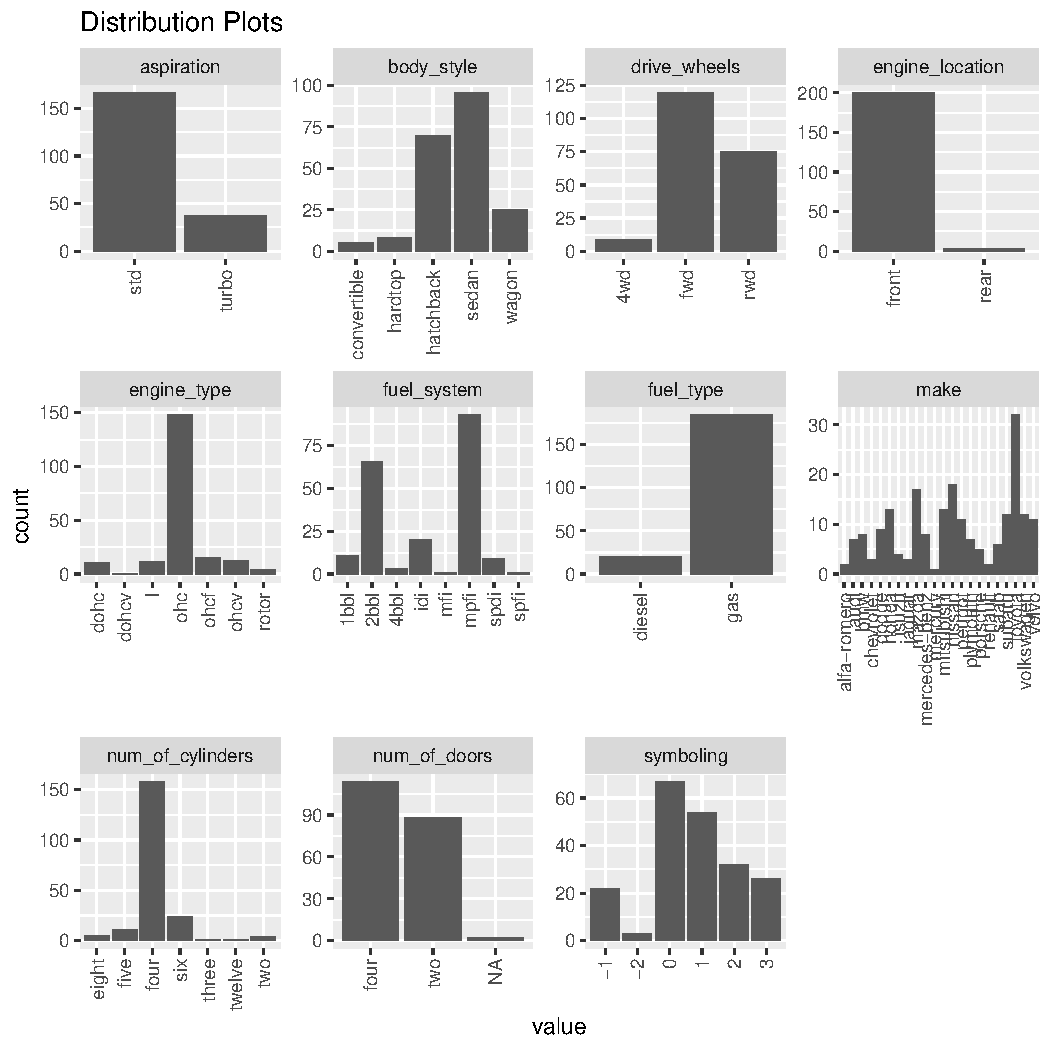
\includegraphics[width=\maxwidth]{figure/barplots_categorical_features-1} \caption[Distribution of all qualitative features in automobile dataset]{Distribution of all qualitative features in automobile dataset}\label{fig:barplots_categorical_features}
\end{figure}

\end{knitrout}
	
\begin{knitrout}
\definecolor{shadecolor}{rgb}{0.969, 0.969, 0.969}\color{fgcolor}\begin{figure}
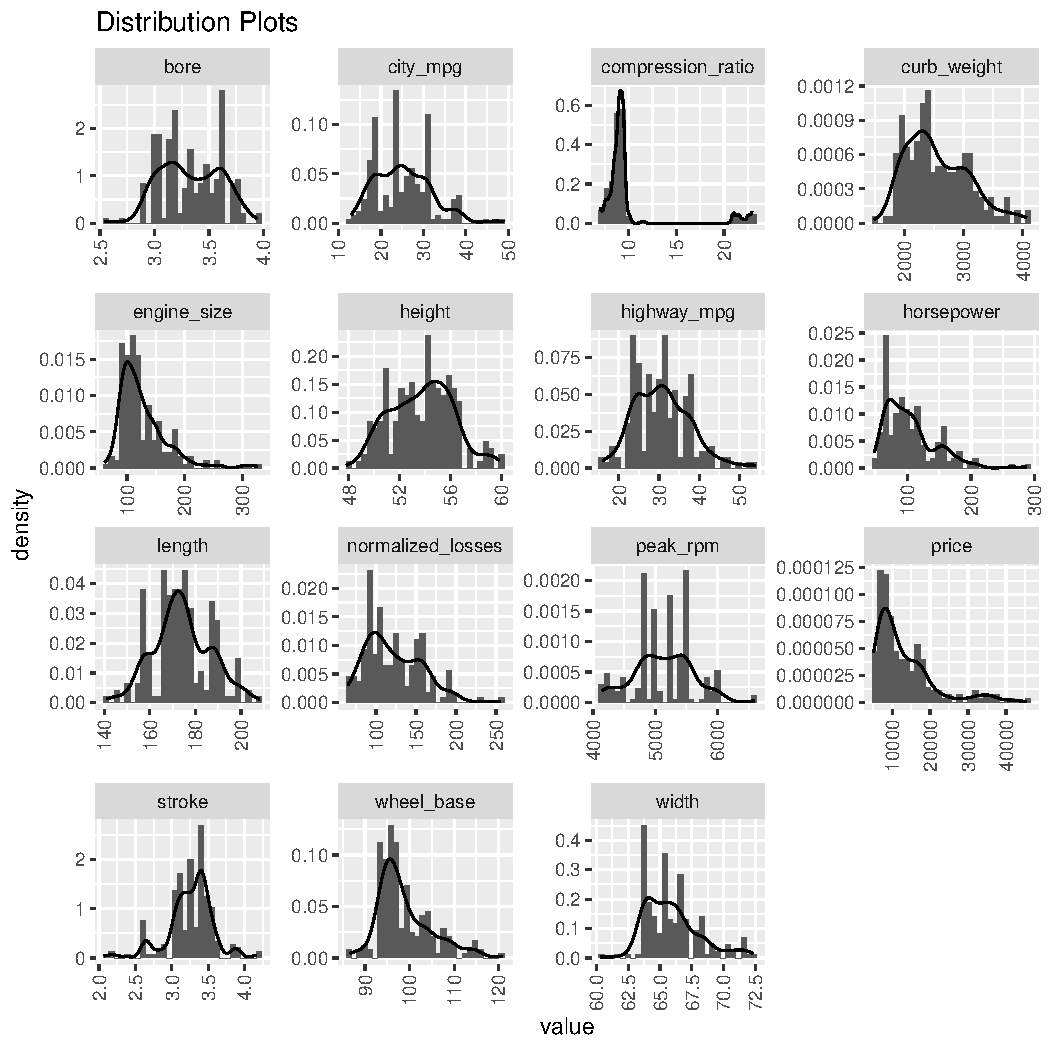
\includegraphics[width=\maxwidth]{figure/hisrograms_numeric_features-1} \caption[Distribution of all quantitative features in automobile dataset]{Distribution of all quantitative features in automobile dataset}\label{fig:hisrograms_numeric_features}
\end{figure}

\end{knitrout}
	
	Figures \ref{fig:barplots_categorical_features} and \ref{fig:hisrograms_numeric_features} show us distributions of categorical and numerical features respectively. In the figure \ref{fig:barplots_categorical_features} we can see the barplots with possibly variables, which the features can take and in the figure \ref{fig:hisrograms_numeric_features} we can see normalized histograms with marked curves, which indicate the kernel density of features.
	
	It is also worth noticing how quantitative features describe the predicted class.
\begin{knitrout}
\definecolor{shadecolor}{rgb}{0.969, 0.969, 0.969}\color{fgcolor}\begin{figure}
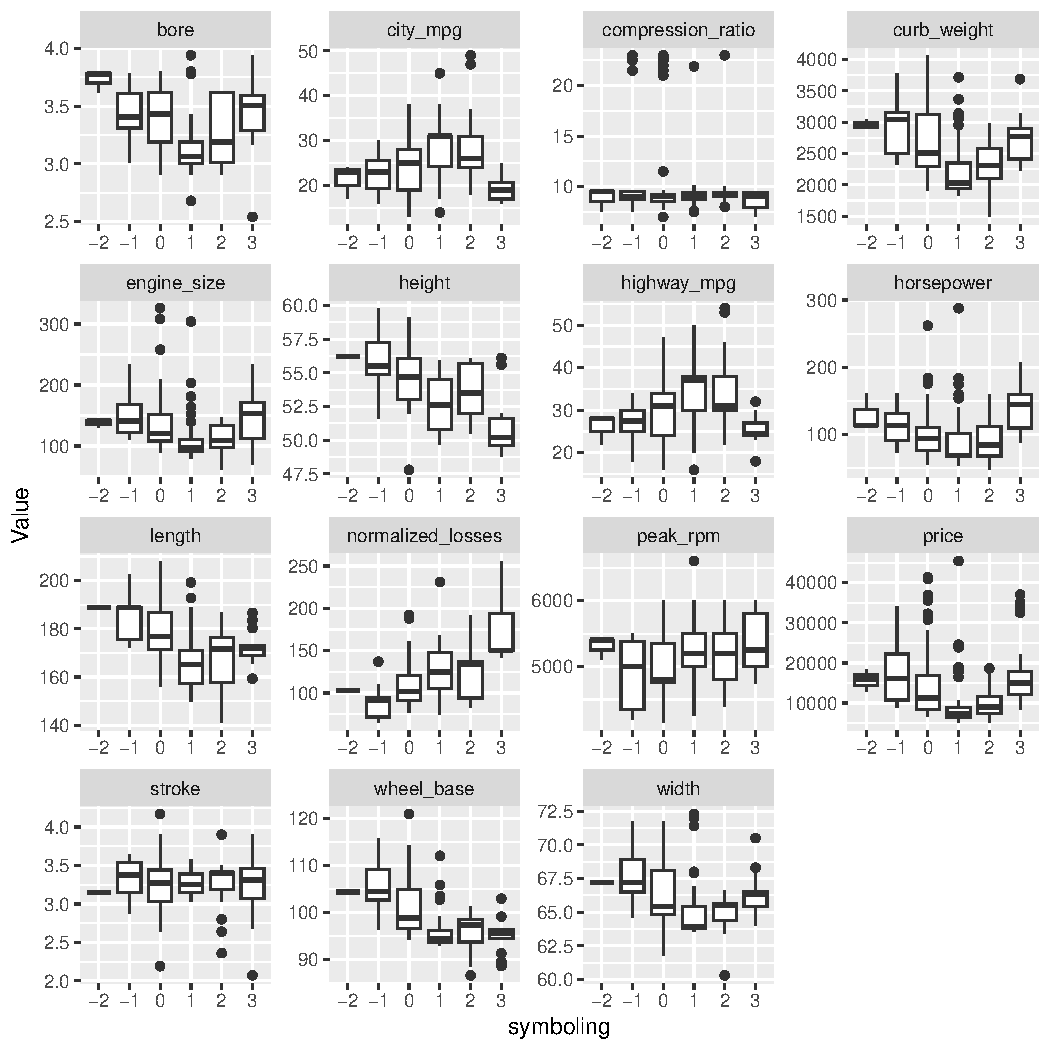
\includegraphics[width=\maxwidth]{figure/quantitative_symboling-1} \caption[Boxplots of description symboling by quantitative features]{Boxplots of description symboling by quantitative features}\label{fig:quantitative_symboling}
\end{figure}

\end{knitrout}
	
	In the figure \ref{fig:quantitative_symboling} we can see that for all features there are is no such a situation, that boxplots are separable. One boxplot can be almost isolated for rare features, like for example variable "-2" for "bore", but in general this approach doesn't provide much information about the predicted value
	
	\subsection{Dealing with missing values}
	
	Let's see the distribution on missing values in our data. Because of many features, we temporarily remove columns with no missing values to better visualize the distribution:
	
\begin{knitrout}
\definecolor{shadecolor}{rgb}{0.969, 0.969, 0.969}\color{fgcolor}\begin{table}

\caption{\label{tab:missing_value_distribution}Distribution of missing values in the dataset}
\centering
\begin{tabular}[t]{l|r|r|r|r|r|r|r|r}
\hline
  & num\_of\_doors & horsepower & peak\_rpm & bore & stroke & price & normalized\_losses & \\
\hline
159 & 1 & 1 & 1 & 1 & 1 & 1 & 1 & 0\\
\hline
33 & 1 & 1 & 1 & 1 & 1 & 1 & 0 & 1\\
\hline
4 & 1 & 1 & 1 & 1 & 1 & 0 & 0 & 2\\
\hline
4 & 1 & 1 & 1 & 0 & 0 & 1 & 1 & 2\\
\hline
2 & 1 & 0 & 0 & 1 & 1 & 1 & 0 & 3\\
\hline
1 & 0 & 1 & 1 & 1 & 1 & 1 & 1 & 1\\
\hline
1 & 0 & 1 & 1 & 1 & 1 & 1 & 0 & 2\\
\hline
 & 2 & 2 & 2 & 4 & 4 & 4 & 40 & 58\\
\hline
\end{tabular}
\end{table}

\end{knitrout}
	Above tabular \ref{tab:missing_value_distribution} shows us pattern of missing values --- the numbers (0, 1) under columns show if there is a missing value of not (1 means not missing, 0 --- missing). The values in the first column show how many records have such a pattern of missing values, for instance 159 records have no missing data. Values in the bottom row describe total sum of missing values of considered column. Numbers in the last column provide number of missing values per pattern. The value in the last row and column provides the total number of missing data in our dataset.
	
	We can see that in our dataset there are 58 missing values, of these 40 occur in the "normalized\_losses" variable. Our dataset is consists of 205 records, so it could be not a good idea to remove all records in which there is at least one missing values, because of this we would loss a lot of information, so we conclude to replace all the missing values by "knn imput" method. 
	
\begin{knitrout}
\definecolor{shadecolor}{rgb}{0.969, 0.969, 0.969}\color{fgcolor}\begin{kframe}
\begin{verbatim}
## [1] 40
\end{verbatim}
\end{kframe}
\end{knitrout}
	

	
	\subsection{Descriptive analysis}
	

			\begin{table}[ht]
			
			%\begin{flushleft}
			\centering
			
			\caption{Values of statistics  for each quantitative column in the dataset.} % title of Table	
			\begin{tabular}{|c |c |c| c | c| c|c| c |} % centered columns (4 columns)
				
				\hline %inserts double horizontal lines
				 & mean & median & IQR & var & sd & madstat & cv\\ [0.5ex] % inserts table
				%heading
    \hline
    
    
				
        	normalized\_losses & 127  & 122 & 59 & 1330& 36.5 & 30.7 & 28.8\\ \hline 
        	
				wheel\_base & 98.8  & 97 & 7.9
& 35.9& 5.99& 4.65 & 6.07\\ \hline

				length & 174&  173 & 16.9 &153&12.4& 9.62 & 7.1\\ \hline
				
				width & 65.9 & 65.5 & 2.83&4.61& 2.15& 1.68 & 3.26 \\ \hline
				
				height & 53.7 & 54.1 & 3.5 &5.88&2.42 &2 & 4.51\\ \hline
				
				curb\_weight & 2560 & 2410 & 794 &\ensuremath{2.72\times 10^{5}}&522 & 430 & 20.4\\ \hline
				
					engine\_size & 127 &  120&  45 &1740& 41.7& 30.4 & 32.9\\ \hline
					
						bore & 3.33 & 3.31& 0.433&0.0738& 0.272& 0.233 & 8.16\\ \hline
						
							stroke & 3.26 &3.29& 0.3&0.0972& 0.312& 0.226 & 9.57\\ \hline
							
								compression\_ratio & 10.1 & 9 &0.825&15.8& 3.98& 2.34 & 39.2\\ \hline
								
									horsepower &5120 & 5200 & 700&1570& 39.6& 30.4 & 38\\ \hline
									
										peak\_rpm & 5120& 5200&  700 &\ensuremath{2.29\times 10^{5}}& 479& 385 & 9.34\\ \hline
										
											city\_mpg &25.2 & 24& 11&42.9 6.55&6.55& 5.22 & 26\\ \hline
											
												highway\_mpg & 30.8 & 30 &  9.5&47.6& 6.9& 5.48 & 22.4\\ \hline
												
													price &\ensuremath{1.32\times 10^{4}} &\ensuremath{1.03\times 10^{4}} & 8740
&\ensuremath{6.28\times 10^{7}}& 7930&5850 & 60.1\\ \hline
		

			\end{tabular}
			\label{table:statistics1} 
		\end{table}
		
		
		
			\begin{table}[ht]
			
			%\begin{flushleft}
			\centering
			
			\caption{Values of statistics  for each quantitative column in the dataset.} % title of Table	
			\begin{tabular}{|c |c |c| c | c| c|c| c |} % centered columns (4 columns)
				
				\hline %inserts double horizontal lines
				 & Q1 & Q3 & skew. & kurtosis & min & max\\ [0.5ex] % inserts table
				%heading
    \hline
    
    
				
        	normalized\_losses & 95   & 154  & 0.525& -0.231 & 65 & 256\\ \hline 
        	
	 	wheel\_base & 94.5    & 102  & 1.05& 0.941 & 86.6 & 121\\ \hline 
	 	
	 	 length & 166  & 183  & 0.148& -0.149 & 141 & 208\\ \hline 
	 	 	
	 	 	 	width & 64.1    & 66.9  & 0.884& 0.611 & 60.3 & 72.3\\ \hline 
	 	 	 	
	 	 	 	
	 	 	 	 	height & 52   & 55.5  & 0.0753& -0.483 & 47.8 & 59.8\\ \hline 
	 	 	 	 	
	 	 	 	 	
	 	 	 	 	 	curb\_weight & 2140   & 2940  & 0.67& -0.114 & 1490 & 4070\\ \hline 
	 	 	 	 	 	
	 	 	 	 	 	
	 	 	 	 	 	 	engine\_size & 97   & 142  & 1.92& 5.03 & 61 & 326\\ \hline 
	 	 	 	 	 	 	
	 	 	 	 	 	 	
	 	 	 	 	 	 	 	bore & 3.15    & 3.58  & 0.0144& -0.832 & 2.54 & 3.94\\ \hline 
	 	 	 	 	 	 	 	
	 	 	 	 	 	 	 	
	 	 	 	 	 	 	 	
	 	 	 	 	 	 	 	 stroke & 3.11   & 3.41  & -0.694& 2.15 & 2.07 & 4.17\\ \hline 
	 	 	 	 	 	 	 	 	
	 	 	 	 	 	 	 	 	
	 	 	 	 	 	 	 	 	
	 	 	 	 	 	 	 	 	 	compression\_ratio & 8.57   & 9.4  & 2.56& 4.95 & 7 & 23\\ \hline 
	 	 	 	 	 	 	 	 	 	
	 	 	 	 	 	 	 	 	 	
	 	 	 	 	 	 	 	 	 	 	horsepower & 70  & 116  & 1.38& 2.51 & 48 & 288\\ \hline 
	 	 	 	 	 	 	 	 	 	 	
	 	 	 	 	 	 	 	 	 	 	
	 	 	 	 	 	 	 	 	 	 	 	peak\_rpm & 4800    & 5500  & 0.0745& \ensuremath{-7.14\times 10^{-5}} & 4150 & 6600\\ \hline 
	 	 	 	 	 	 	 	 	 	 	 	
	 	 	 	 	 	 	 	 	 	 	 	
	 	 	 	 	 	 	 	 	 	 	 	 	city\_mpg & 19    & 30  & 0.646& 0.489 & 13 & 49\\ \hline 
	 	 	 	 	 	 	 	 	 	 	 	 	
	 	 	 	 	 	 	 	 	 	 	 	 	
	 	 	 	 	 	 	 	 	 	 	 	 	 highway\_mpg & 25    & 34.5  & 0.525& 0.354 & 16 & 54\\ \hline 
	 	 	 	 	 	 	 	 	 	 	 	 	 	
	 	 	 	 	 	 	 	 	 	 	 	 	 	
	 	 	 	 	 	 	 	 	 	 	 	 	 	 	price & 7770    & \ensuremath{1.65\times 10^{4}}  & 1.78& 3.06 & 5120 & \ensuremath{4.54\times 10^{4}}\\ \hline 
	 	 	 	 	 	 	 	 	 	 	 	 	 	 	
	 	 	 	 	 	 	 	 	 	 	 	 	 	 	
 	 	 	 	 	 	 	 	

	\end{tabular}
			\label{table:statistics2} 
		\end{table}

	

	
	
	In tables \ref{table:statistics1} and \ref{table:statistics2} we present values of mean, median, interquartile range (IQR), variance (var), standard deviation (sd), mean-absolute deviation (madstat), coefficient of variation (cv), first quartile (Q1), third quartile (Q3), skweness (skew.), kurtosis, minimal value (min) and maximal value (max). Looking at the tables we can conclude:
	\begin{enumerate}
	\item The data on normalized losses appears to have a moderately spread distribution with a relatively low coefficient of variation, indicating a moderate level of relative variability. The distribution of normalized losses is slightly right-skewed (positive skewness) with a moderate kurtosis. The majority of the data falls within the interquartile range (IQR), and there are potential outliers on the higher end, as indicated by the relatively large maximum value.
	
	\item The wheel base data is more tightly distributed compared to normalized losses, with a low coefficient of variation suggesting lower relative variability. The wheel base data is right-skewed with a positive kurtosis, suggesting a distribution with a tail on the right. The majority of the data is within the IQR, and there are potential outliers on the higher end.
	
	\item Similar to wheel base, the length data has a relatively low coefficient of variation, indicating a moderate level of relative variability. The length data has a relatively symmetric distribution with a slight right skewness and negative kurtosis. The majority of the data falls within the IQR, and there are potential outliers on the higher end.
	
	
	\item The width data is relatively tightly distributed with a low coefficient of variation. The width data is right-skewed with positive kurtosis. The majority of the data is within the IQR, and there are potential outliers on the higher end.
	
	
	\item The height data shows a moderate level of relative variability. The height data is slightly right-skewed with a negative kurtosis. The majority of the data is within the IQR, and there are potential outliers on the lower end.
	
	
	\item Curb weight data has a higher coefficient of variation, indicating a higher level of relative variability. Curb weight data is right-skewed with a moderate kurtosis. The majority of the data is within the IQR, and there are potential outliers on the higher end.
	
	
	\item Engine size data has moderate relative variability. The engine size data is right-skewed with a high positive kurtosis, indicating a distribution with a heavy tail on the right. The majority of the data is within the IQR, and there are potential outliers on the higher end.
	
	
	\item Bore data is relatively tightly distributed with a higher coefficient of variation. The bore data is nearly normally distributed with low skewness and negative kurtosis. The majority of the data falls within the IQR.
	
	
	\item Stroke data has a higher coefficient of variation, indicating higher relative variability. Stroke data is left-skewed with a positive kurtosis, suggesting a distribution with a tail on the left. The majority of the data is within the IQR.
	
	
	\item Compression ratio data has a high coefficient of variation, suggesting a high level of relative variability. Compression ratio data is highly right-skewed with a high positive kurtosis. The majority of the data is within the IQR, and there are potential outliers on the higher end.
	
	
	\item Horsepower data has moderate relative variability. Horsepower data is right-skewed with positive kurtosis. The majority of the data is within the IQR, and there are potential outliers on the higher end.
	
	
	\item Peak RPM data is relatively tightly distributed with a low coefficient of variation. Peak RPM data is slightly right-skewed with low kurtosis. The majority of the data is within the IQR.
	
	
	\item City miles per gallon data has relatively low variability. City miles per gallon data is right-skewed with positive kurtosis. The majority of the data is within the IQR, and there are potential outliers on the higher end.
	
	
	\item Highway miles per gallon data has moderate variability. Highway miles per gallon data is right-skewed with positive kurtosis. The majority of the data is within the IQR, and there are potential outliers on the higher end.
	
	
	\item Price data has a high coefficient of variation, indicating a high level of relative variability. The price data is significantly right-skewed with a high positive kurtosis, indicating a distribution with a heavy tail on the right. The majority of the data falls within the interquartile range (IQR), and there are potential outliers on the higher end. This suggests that the prices are concentrated in a relatively narrow range for the majority of the vehicles, with a few high-priced outliers.

	\end{enumerate}



	
	
\begin{knitrout}
\definecolor{shadecolor}{rgb}{0.969, 0.969, 0.969}\color{fgcolor}\begin{figure}
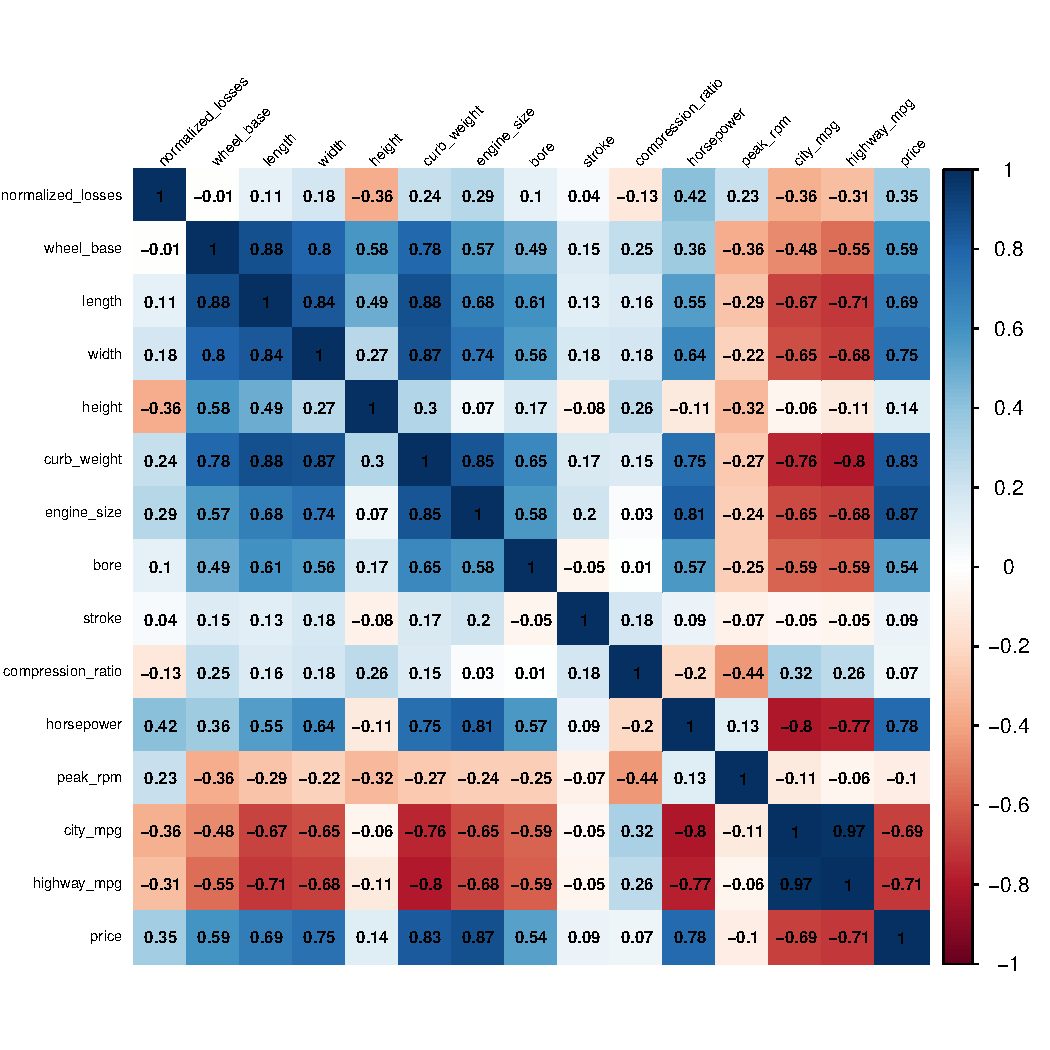
\includegraphics[width=\maxwidth]{figure/corr_plot-1} \caption[Correlation heatmap for all features]{Correlation heatmap for all features}\label{fig:corr_plot}
\end{figure}

\end{knitrout}
	
	
	In figure \ref{fig:corr_plot} we present a heatmap containing correlation coefficients between all the quantitative features. Analysing it we can conclude that:
	\begin{enumerate}
	
\item we observe strong positive correlations between: city\_mpg and highway\_mpg, wheel\_base and length, engine\_size and horsepower, length and width, length and curb\_width, engine\_size and curb\_width.
\item we observe moderate negative correlations between: peak\_rpm and price, horsepower and price, compression\_ratio and highway\_mpg, length and highway\_mpg, curb\_weight and city\_mpg.
\item we can conclude that the horsepower and engine\_size show a strong positive correlation of 0.78, indicating that vehicles with larger engines tend to have higher horsepower. Columns curb\_weight and engine\_size also exhibit a strong positive correlation of 0.78, suggesting that heavier vehicles tend to have larger engines.There is a noticeable negative correlation between highway\_mpg and several other features, indicating that as certain vehicle attributes increase, fuel efficiency on the highway tends to decrease.
\item we have also observed that the city\_mpg and highway\_mpg are pretty correlated, the coefficient is close to 1, so we are not going to consider city\_mpg variable in further analysis
	\end{enumerate}
	
	\subsection{Normality test}
	
		\begin{table}[ht]
			
			%\begin{flushleft}
			\centering
			
			\caption{Values of statistic of p--value of performed Shapiro Wilk test for normality for each quantitative column in the dataset.} % title of Table	
			\begin{tabular}{|c |c |c|} % centered columns (4 columns)
				
				\hline %inserts double horizontal lines
				 & p -- value & statistic \\ [0.5ex] % inserts table
				%heading
    \hline
				
         normalized\_losses & $7.145 \cdot 10^{-6}$ &  0.95665\\ \hline     
				wheel\_base & $ 6.726 \cdot 10^{-10}$  & 0.90841   \\ \hline
				length & 0.01149 &  0.98232 \\ \hline
				width & $6.354 \cdot 10^{-9}$ & 0.92207  \\ \hline
				height & 0.01814 & 0.98365 \\ \hline
				curb\_weight & $2.741 \cdot 10^{-6}$ & 0.95259\\ \hline
					engine\_size & $3.225 \cdot 10^{-14}$ &  0.82909\\ \hline
						bore & $ 8.366 \cdot 10^{-5}$ & 0.96623\\ \hline
							stroke & $8.31 \cdot 10^{-8}$ & 0.93608 \\ \hline
								compression\_ratio & $2.2 \cdot 10^{-16}$ & 0.49886 \\ \hline
									horsepower & $1.972 \cdot 10^{-11}$ & 0.884 \\ \hline
										peak\_rpm & 0.0002378 & 0.96996\\ \hline
											city\_mpg & $8.572 \cdot 10^{-6}$ & 0.9574\\ \hline
												highway\_mpg & 0.0007151 &  0.9737 \\ \hline
													price &$1.899 \cdot 10^{-15}$ &0.79994 \\ \hline
		

			\end{tabular}
			\label{table:shapiro} 
		\end{table}
		
		
		The table \ref{table:shapiro} presents the results of the Shapiro--Wilk test for normality conducted on various quantitative columns in the dataset. The test assesses whether the data in each column follows a normal distribution. The key statistics provided are the p--values and test statistics. Here are the conclusions based on the results:
\begin{enumerate}
\item normalized\_losses -- the p-value is extremely small ($7.145 \cdot 10^{-6}$), indicating that the data for wheel\_base is not normally distributed,

\item wheel\_base -- the p-value is extremely small ($6.726 \cdot 10^{-10}$), indicating that the data for wheel\_base is not normally distributed,

\item length -- the p-value (0.01149) is less than the typical significance level of 0.05, suggesting that the data for length is not normally distributed.

\item width -- the p-value is very small ($6.354 \cdot 10^{-9}$), indicating that the data for width is not normally distributed.

\item height -- the p-value (0.01814) is less than 0.05, suggesting that the data for height is not normally distributed.

\item curb\_weight -- the p-value is small ($2.741 \cdot 10^{-6}$), indicating that the data for curb\_weight is not normally distributed.

\item engine\_size -- the p-value is extremely small ($3.225 \cdot 10^{-14}$), indicating that the data for engine\_size is not normally distributed.

\item bore -- the p--value is small ($8.366 \cdot 10^{-5}$), suggesting that the data for bore is not normally distributed.

\item stroke -- the p-value is small ($8.31 \cdot 10^{-8}$), indicating that the data for stroke is not normally distributed.

\item compression\_ratio -- the p-value is extremely small ($2.2 \cdot 10^{-16}$), indicating that the data for compression\_ratio is not normally distributed.

\item horsepower -- the p-value is very small ($1.972 \cdot 10^{-11}$), indicating that the data for horsepower is not normally distributed.

\item peak\_rpm -- the p-value (0.0002378) is less than 0.05, suggesting that the data for peak\_rpm is not normally distributed.

\item city\_mpg -- the p-value is small ($8.572 \cdot 10^{-6}$), indicating that the data for city\_mpg is not normally distributed.

\item highway\_mpg -- the p-value (0.0007151) is less than 0.05, suggesting that the data for highway\_mpg is not normally distributed.

\item price -- the p-value is extremely small ($1.899 \cdot 10^{-15}$), indicating that the data for price is not normally distributed.

\end{enumerate}

In summary, based on the Shapiro--Wilk test results, none of the quantitative columns in the dataset appear to follow a normal distribution. This information is important for choosing appropriate statistical analyses, as some methods assume normality in the data. 


\begin{knitrout}
\definecolor{shadecolor}{rgb}{0.969, 0.969, 0.969}\color{fgcolor}\begin{figure}
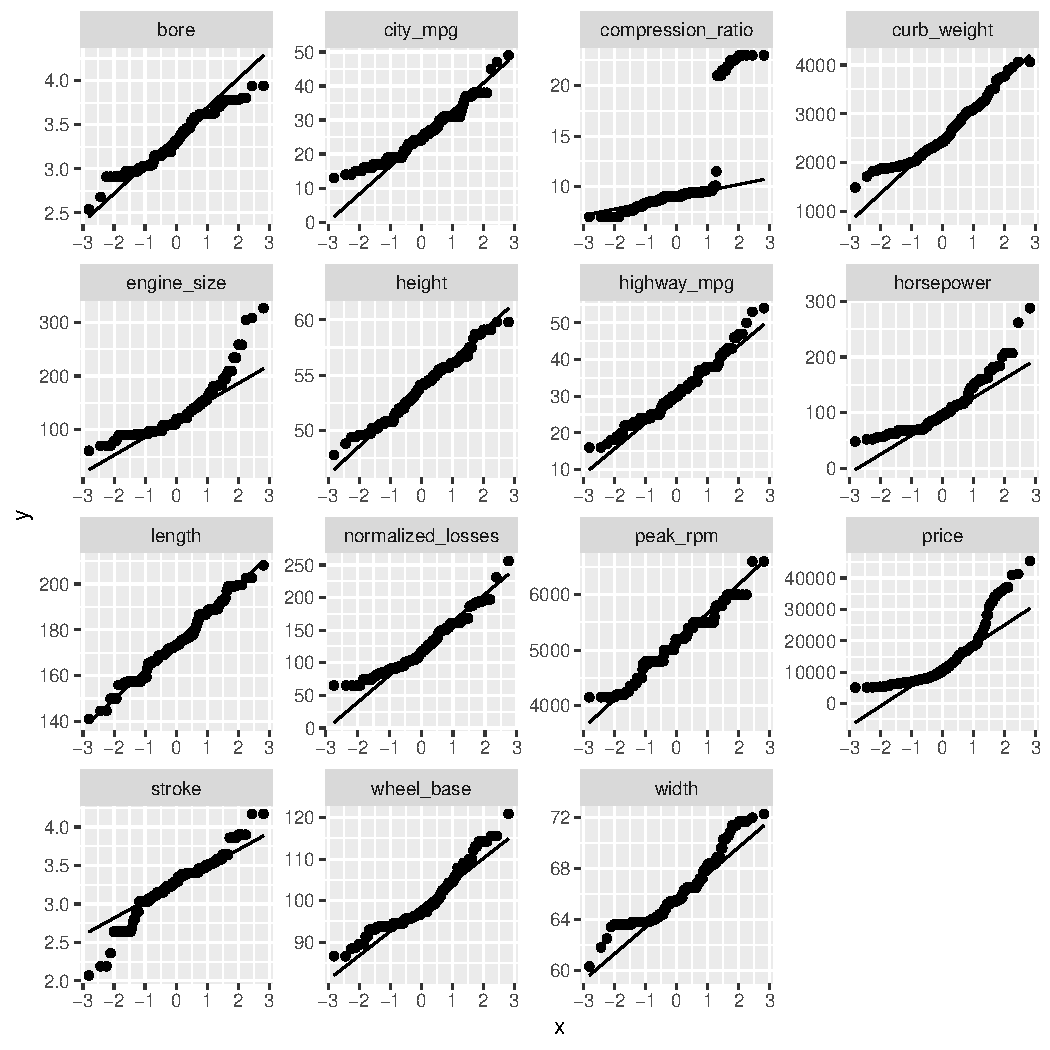
\includegraphics[width=\maxwidth]{figure/qqplot_EDA-1} \caption[Q-Q plots for all the quantitative features]{Q-Q plots for all the quantitative features.}\label{fig:qqplot_EDA}
\end{figure}

\end{knitrout}
	
In figure \ref{fig:qqplot_EDA} we present Q--Q plots for all the quantitative features in the dataset. Based on them, we can assess normality of data. What we can observe is the fact, that the length looks to be the closest to the normal distribution, the rest of the columns do not cover the line. Summing up the results obtained from the Shapiro--Wilk test and Q--Q plots we conclude that none of the features follows the normal distribution.
	

	



	
	\section{Classification}\label{sec:classification}
In this section, we explore various classification methods and compare them to gain a deeper understanding of our dataset.
	
Firstly, we will begin with data preparation to determine whether our data should be standardized or if other modifications are necessary. Next, we will apply different classification methods, including linear regression, logistic regression, k–nearest neighbors, linear discriminant analysis, quadratic discriminant analysis, decision tree, random forest, and support vector machines.
	
	We will divide our dataset into training and test sets in a 0.85:0.15 proportion. The test set will be exclusively used in section \ref{sec:comparison} for the summary of accuracy of all considered classification methods. To choose the best parameters (e.g., the number of neighbors in k-–NN) among all studied methods, we will employ a 5-–fold Cross–-Validation assessment procedure in the training set.
	
	In section \ref{sec:data_preparation}, we will use the Random Forest method to investigate the most important features for the predicted class. The selected features will be utilized in each model. In addition to this approach, we will build a model that includes all features (those we won't delete from the dataset, for example, due to a variance approximately equal to 0). All obtained results will be compared in section \ref{sec:comparison}.
	


	\subsection{Data preparation}\label{sec:data_preparation}
	In this subsection, we will address data preparation to ensure our data is ready for constructing the classification models.
	
	Firstly, it is important to note that in our target variable, "symboling," there are only three instances where the "symboling" has a value equal to -2, as illustrated in figure \ref{fig:barplots_categorical_features}. Building a meaningful model with such limited data for this variable is challenging. Therefore, we have chosen to exclude these records from our dataset, as the loss of information is minimal.
	
	

	

\begin{knitrout}
\definecolor{shadecolor}{rgb}{0.969, 0.969, 0.969}\color{fgcolor}\begin{figure}
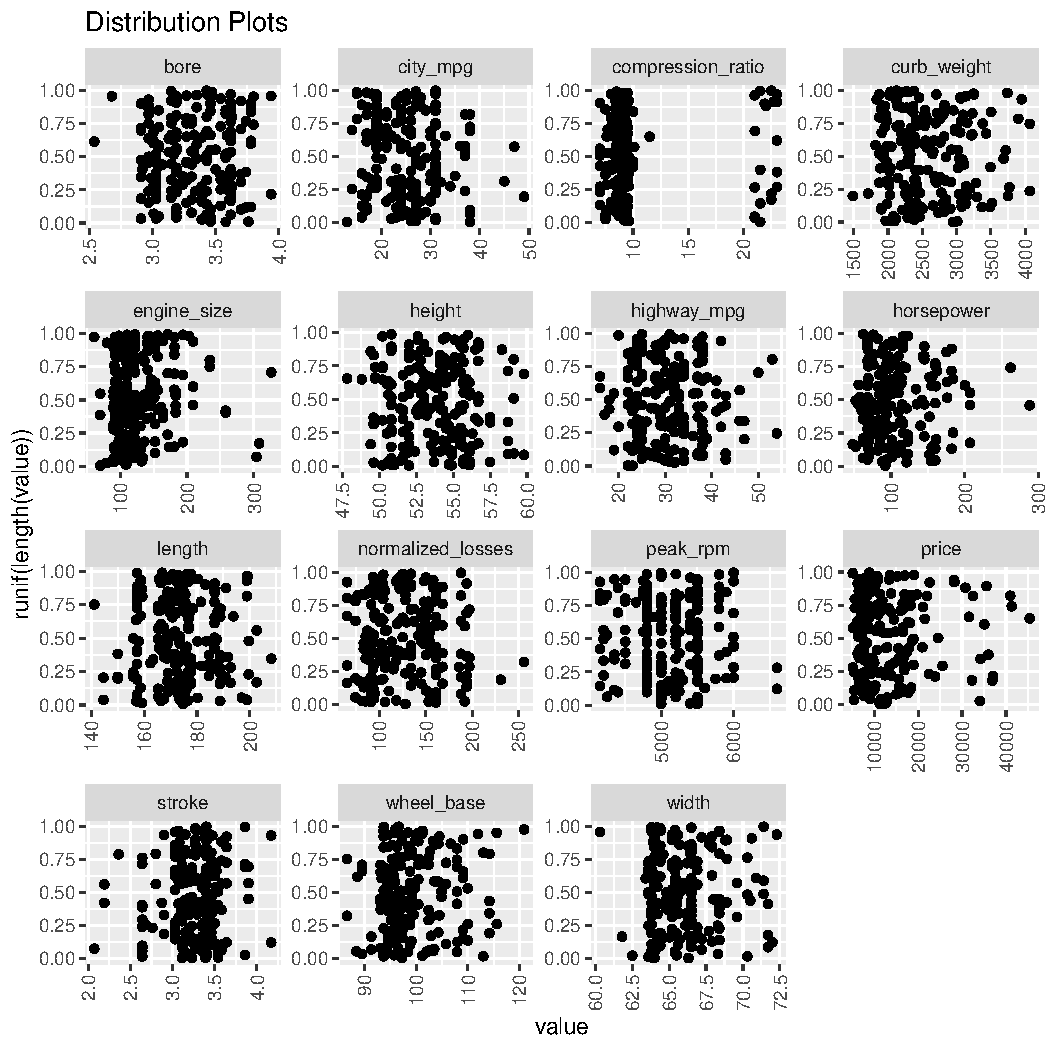
\includegraphics[width=\maxwidth]{figure/distribution_quantitative-1} \caption[Distribution of quantitative variables]{Distribution of quantitative variables}\label{fig:distribution_quantitative}
\end{figure}

\end{knitrout}
In figure \ref{fig:distribution_quantitative}, the distribution of all quantitative features in our data is illustrated. The values of individual variables are marked on the x-axis, while the y-axis represents values from a uniform distribution. This approach provides a better visualization of the relationships among variables.

Upon inspecting the distribution plots, we have determined that it is worthwhile to binarize the "compression\_ratio" feature. This decision is based on the clear delineation of two classes observed in the variable values. Additionally, we plan to standardize all quantitative features to homogenize the scale of the data.
	


	

\begin{knitrout}
\definecolor{shadecolor}{rgb}{0.969, 0.969, 0.969}\color{fgcolor}\begin{kframe}
\begin{verbatim}
## 
##  low high 
##  181   20
\end{verbatim}
\end{kframe}
\end{knitrout}
	

	
	
	Let us compare boxplots of standardized and non--standardized data:
	
\begin{knitrout}
\definecolor{shadecolor}{rgb}{0.969, 0.969, 0.969}\color{fgcolor}\begin{figure}
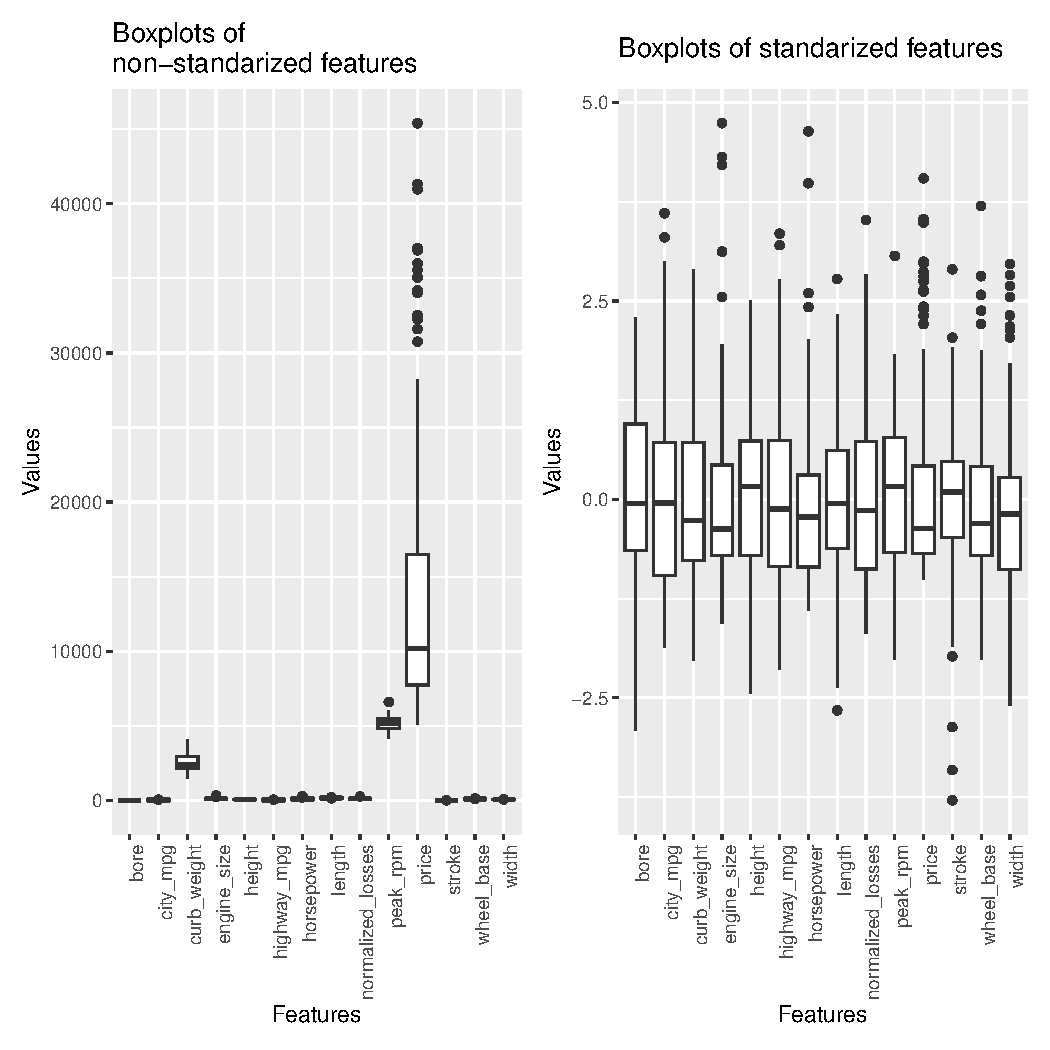
\includegraphics[width=\maxwidth]{figure/Boxplots_of_standarized_and_non_standarized_quantitative_features-1} \caption[Boxplots of all standarized and non-standarized quantitative features]{Boxplots of all standarized and non-standarized quantitative features}\label{fig:Boxplots_of_standarized_and_non_standarized_quantitative_features}
\end{figure}

\end{knitrout}
	
	
In figure \ref{fig:Boxplots_of_standarized_and_non_standarized_quantitative_features}, we can observe that the boxplots depicting standardized quantitative features provide more informative insights compared to those of the non--standardized features. Notably, it is observed that almost all features exhibit outliers, with the exception of the "stroke" feature. These outliers predominantly occur on the right side of the distribution. Furthermore, a recurring pattern is discerned, indicating a prevalent right--skewed distribution in the data.
	
Our next step is to split the dataset into two parts: one containing the "symboling" column (our class) and the other containing the remaining features.

	

	
	Now, we are examining features that offer minimal information. To achieve this, we will identify features with variances close to zero. These features are not conducive to constructing models, especially when our predicted value consists of six classes, as they exhibit nearly constant values. Feature for which the variance is equal near to zero is:
	
\begin{knitrout}
\definecolor{shadecolor}{rgb}{0.969, 0.969, 0.969}\color{fgcolor}\begin{kframe}
\begin{verbatim}
## [1] "engine_location"
\end{verbatim}
\end{kframe}
\end{knitrout}
	

	
	We conclude that for high correlated features to leave one of them. We will consider groups of features for which correlation is larger than 0.9. In the heat map \ref{fig:corr_plot}, which describes correlations among all features we can see that for quantitative variables: "city\_mpg" and "highway\_mpg" the correlation is equal to 0.97. So we decided to remove "city\_mpg" from the dataset.
	

	
	We also use one--hot encoding to avoid some problems for considered classification models. One-hot encoding is a good approach to represent categorical type of features. Most of the classification models can not manage with such categorical values. 
	
	Before we move on to the classification section, we divide our dataset into training and test set. First of them we will use to build the classification model and the second one is needed to getting conclusion of results. We will use test set only in \ref{sec:comparison} section. We will calculate estimated accuracy of all considered classification problems using 5--fold Cross--Validation assessment method. Train and test subsets are divided into 0.85:0.15 proportions.
	

	


	
	Our next step is selection of the most important features, which we will use to build one of the model in each of considered classification method. To do this we  use feature elimination based on Random Forest approach. We will consider subsets which contains of between 1 and 50 features

	Outcome of the Random Forest approach for selecting the most important features is as follows:
\begin{knitrout}
\definecolor{shadecolor}{rgb}{0.969, 0.969, 0.969}\color{fgcolor}\begin{kframe}
\begin{verbatim}
## [1] "normalized_losses" "wheel_base"        "height"           
## [4] "num_of_doors.two"
\end{verbatim}
\end{kframe}
\end{knitrout}
	Now let see the accuracy results for considered selecting subsets of features:
\begin{knitrout}
\definecolor{shadecolor}{rgb}{0.969, 0.969, 0.969}\color{fgcolor}\begin{kframe}
\begin{verbatim}
##         1         2         3         4         5         6         7         8 
## 0.7335109 0.8249213 0.8308381 0.8530603 0.8063248 0.8314229 0.8321173 0.8495274 
##         9        10        11        12        13        14        15        16 
## 0.8495618 0.8491942 0.8491942 0.8377563 0.8377563 0.8374295 0.8263592 0.8259916 
##        17        18        19        20        21        22        23        24 
## 0.8142269 0.8189981 0.8256648 0.8312203 0.8253380 0.8364491 0.8253380 0.8308935 
##        25        26        27        28        29        30        31        32 
## 0.8430603 0.8371027 0.8245537 0.8298168 0.8242269 0.8353724 0.8359916 0.8242269 
##        33        34        35        36        37        38        39        40 
## 0.8356648 0.8239001 0.8363592 0.8412547 0.8301092 0.8304360 0.8356648 0.8131158 
##        41        42        43        44        45        46        47        48 
## 0.8177253 0.8190390 0.8242269 0.8245945 0.8236077 0.8291632 0.8183445 0.8180521 
##        49        50        73 
## 0.8354132 0.8301092 0.8236077
\end{verbatim}
\end{kframe}
\end{knitrout}
	
	We get maximal value of accuracy for 4 features, but for all values from considered interval the accuracy is quite large --- above 0.8 (apart from case of 1 feature).

We will use the optimal features to build the model in each classification method.


	
	\subsection{Linear regression}\label{sec:linear_regression}
	In this subsection we apply the linear regression to predict "symboling" variable. We will use "one versus rest" approach, to deal with multiple value of classes in our predicted variable. The "one versus rest" approach is based on binarize the predicted value, what lead to consider multiple tasks of binarize problem. 
	
Our predicted class consists of five values. Therefore, we decompose the linear regression problem into five binary problems.
	
	Let us build the model, which consists all quantitative features and let's check their confusion matrix.
	

	
\begin{knitrout}
\definecolor{shadecolor}{rgb}{0.969, 0.969, 0.969}\color{fgcolor}\begin{kframe}
\begin{verbatim}
##    -1  0  1  2  3
## -1 15  4  4  1  6
## 0   3 44 12 15  5
## 1   1  9 30 12 14
## 2   0  0  0  0  2
## 3   0  0  0  0  2
\end{verbatim}
\end{kframe}
\end{knitrout}
	And now let see the accuracy for this method:
	
\begin{knitrout}
\definecolor{shadecolor}{rgb}{0.969, 0.969, 0.969}\color{fgcolor}\begin{kframe}
\begin{verbatim}
## [1] 0.5083799
\end{verbatim}
\end{kframe}
\end{knitrout}
	
	And the results for the most important features:
	
\begin{knitrout}
\definecolor{shadecolor}{rgb}{0.969, 0.969, 0.969}\color{fgcolor}\begin{kframe}
\begin{verbatim}
##    -1  0  1  2  3
## -1  0  1  2  0  0
## 0  19 50 18  9  0
## 1   0  6 26 19 23
## 2   0  0  0  0  0
## 3   0  0  0  0  0
\end{verbatim}
\end{kframe}
\end{knitrout}

\begin{knitrout}
\definecolor{shadecolor}{rgb}{0.969, 0.969, 0.969}\color{fgcolor}\begin{kframe}
\begin{verbatim}
## [1] 0.4393064
\end{verbatim}
\end{kframe}
\end{knitrout}

	
	

For the original features the model achieved an accuracy of approximately 0.5083799.
The confusion matrix indicates that the model struggled to accurately predict instances across all classes, with notable misclassifications in various cells.
For the most important features the model achieved an accuracy of approximately 0.4393064.
The confusion matrix for the most important features shows more pattern of misclassifications, and the accuracy is significantly larger for whole dataset.
Both models seem to have similar performance.
Further analysis, feature engineering, or trying different models may be needed to improve classification performance.
	\subsection{Logistic regression}
	Logistic regression also requires from us dividing the multi--classification task into multiple binary--classification tasks ("one versus rest" approach). So as in \ref{sec:linear_regression} subsection we divide the problem into six tasks and similarly we use only quantitative features to fit the model. 

	
\begin{knitrout}
\definecolor{shadecolor}{rgb}{0.969, 0.969, 0.969}\color{fgcolor}\begin{kframe}
\begin{verbatim}
##    -1  0  1  2  3
## -1 13  8  9  3  5
## 0   3 38 13 17  9
## 1   4 12 29 20 14
## 2   1  1  5 12  5
## 3   1  1  5 12  5
\end{verbatim}
\end{kframe}
\end{knitrout}
	And now let see the accuracy for this method:
\begin{knitrout}
\definecolor{shadecolor}{rgb}{0.969, 0.969, 0.969}\color{fgcolor}\begin{kframe}
\begin{verbatim}
## [1] 0.3959184
\end{verbatim}
\end{kframe}
\end{knitrout}
	
	Now let us see results for the most important features:
	
\begin{knitrout}
\definecolor{shadecolor}{rgb}{0.969, 0.969, 0.969}\color{fgcolor}\begin{kframe}
\begin{verbatim}
##    -1  0  1  2  3
## -1 16  1  0  0  0
## 0   3 50 19  9  0
## 1   0  6 27 19 23
## 2   0  0  0  0  0
## 3   0  0  0  0  0
\end{verbatim}
\end{kframe}
\end{knitrout}

\begin{knitrout}
\definecolor{shadecolor}{rgb}{0.969, 0.969, 0.969}\color{fgcolor}\begin{kframe}
\begin{verbatim}
## [1] 0.5375723
\end{verbatim}
\end{kframe}
\end{knitrout}
	
For the original features the model achieved an accuracy of approximately 0.3959184.
The confusion matrix indicates difficulties in accurately predicting instances across all classes. The model tends to misclassify instances, especially in predicting class 1.
For the the most important features the model achieved an improved accuracy of approximately 0.5375723 when using the most important features.
The confusion matrix for the most important features shows better performance, with fewer misclassifications compared to the model with original features.
Logistic regression with the most important features outperforms logistic regression with the original features.
The accuracy improvement suggests that the selection of the most important features has a positive impact on the model's predictive performance.

	
	\subsection{k-Nearest Neighbors (k-NN)}
	
	K-NN method is based on k nearest neighbors to a given data point and it takes the majority vote to classify the data point.
	
Let us apply kNN algorithm to our whole dataset and for most important features. 

	



\begin{knitrout}
\definecolor{shadecolor}{rgb}{0.969, 0.969, 0.969}\color{fgcolor}\begin{figure}
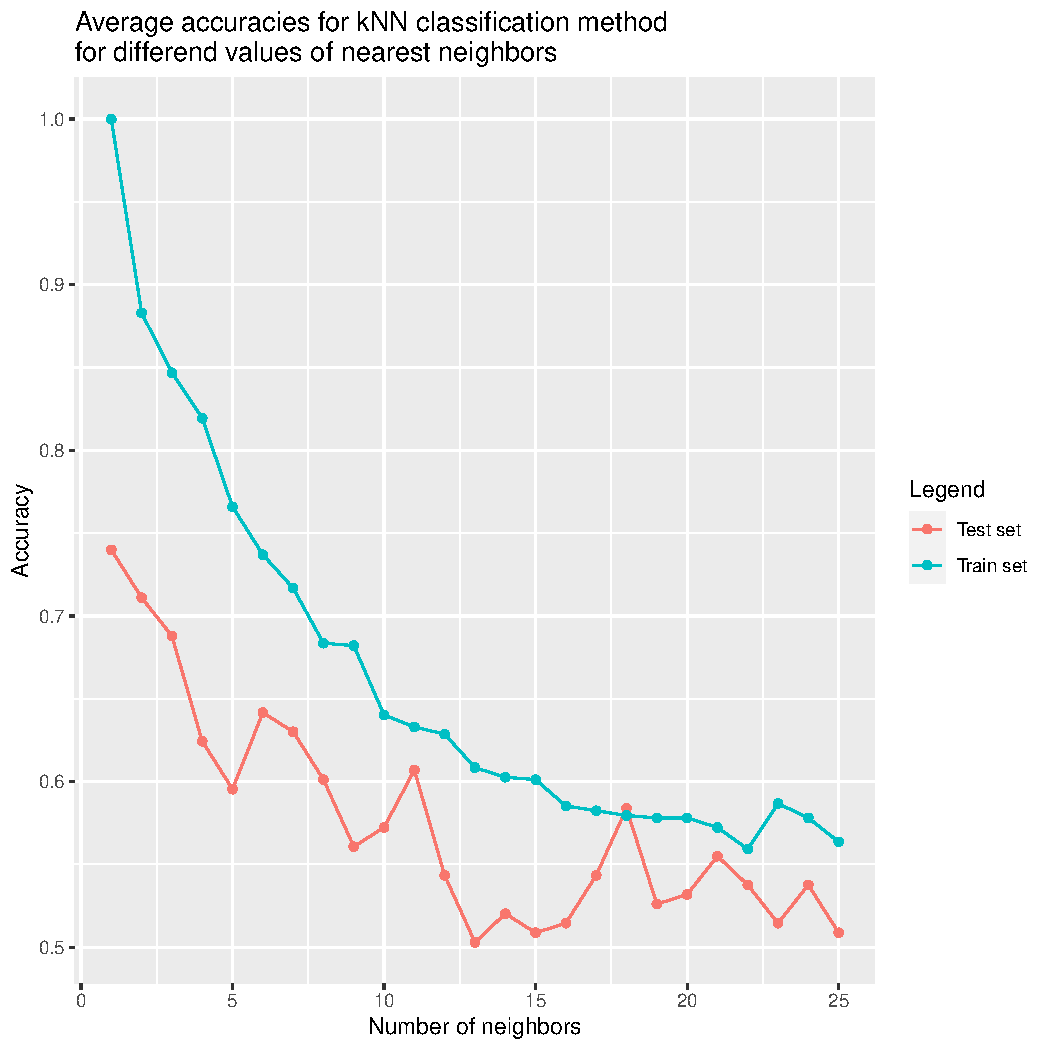
\includegraphics[width=\maxwidth]{figure/knn_results-1} \caption[Accuracies comparison for train and test sets (summarized results for 5-fold C-V)]{Accuracies comparison for train and test sets (summarized results for 5-fold C-V)}\label{fig:knn_results}
\end{figure}

\end{knitrout}
	


\begin{knitrout}
\definecolor{shadecolor}{rgb}{0.969, 0.969, 0.969}\color{fgcolor}\begin{figure}
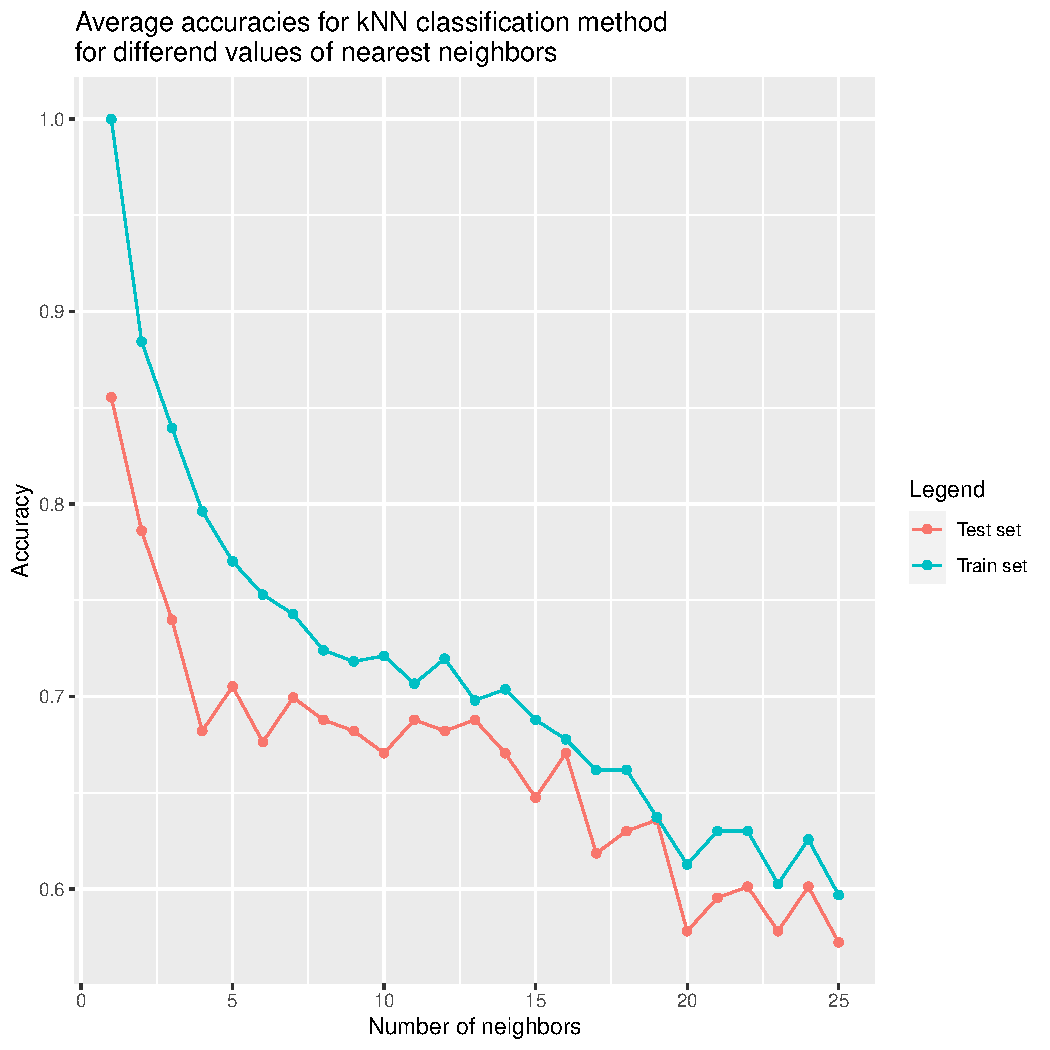
\includegraphics[width=\maxwidth]{figure/knn_results2-1} \caption[Accuracies comparison for train and test sets (summarized results for 5-fold C-V) for selected features]{Accuracies comparison for train and test sets (summarized results for 5-fold C-V) for selected features}\label{fig:knn_results2}
\end{figure}

\end{knitrout}

In figures \ref{fig:knn_results} and \ref{fig:knn_results2} we can see accuracy for train and test sets (summarized for 5-fold Cross-Validation assessment method) for different value of number of nearest neighbors --- k, for whole dataset --- \ref{fig:knn_results} and for selected features --- \ref{fig:knn_results2}. As we see, in the charts, for 1 nearest neighbors the accuracy for train set is equal to 1 (for whole dataset and for selected features) and for test sets accuracies are the largest for 1 nearest neighbors, both for whole dataset and for selected features. We can see that the more number of nearest neighbors are, the less (in general) the accuracies for train and test sets are, for whole dataset and selected features. So we conclude that the optimal number of nearest neighbors is equal to 1.


	\subsection{Linear Discriminant Analysis (LDA)}

In this section we will apply linear discriminant analysis to our dataset.



We obtained such confusion matrix for 5-fold Cross-Validation: 

\begin{knitrout}
\definecolor{shadecolor}{rgb}{0.969, 0.969, 0.969}\color{fgcolor}\begin{kframe}
\begin{verbatim}
##    -1  0  1  2  3
## -1 15  2  4  0  1
## 0   3 42  6  3  0
## 1   0  9 29  5  3
## 2   0  3  4 20  4
## 3   1  1  3  0 15
\end{verbatim}
\end{kframe}
\end{knitrout}

\begin{knitrout}
\definecolor{shadecolor}{rgb}{0.969, 0.969, 0.969}\color{fgcolor}\begin{kframe}
\begin{verbatim}
## [1] 0.699422
\end{verbatim}
\end{kframe}
\end{knitrout}

	Now let us see results for the most important features:
	
\begin{knitrout}
\definecolor{shadecolor}{rgb}{0.969, 0.969, 0.969}\color{fgcolor}\begin{kframe}
\begin{verbatim}
##    -1  0  1  2  3
## -1 17  4  1  0  0
## 0   2 47 15  9  0
## 1   0  4 16 11  5
## 2   0  0  9  2  3
## 3   0  2  5  6 15
\end{verbatim}
\end{kframe}
\end{knitrout}

\begin{knitrout}
\definecolor{shadecolor}{rgb}{0.969, 0.969, 0.969}\color{fgcolor}\begin{kframe}
\begin{verbatim}
## [1] 0.5606936
\end{verbatim}
\end{kframe}
\end{knitrout}

During building the models we have to remove constant columns from a dataframe, because LDA in R language can not have constant column. We assume that this affect not so much for results, because in every split (in 5-fold Cross-Validation) there were a little number of constant columns (between 1-4). Fixed columns exist in case when there is no instance of certain value for qualitative values (because of one-hot encoding).



For original features the model achieved an accuracy of approximately 0.699422.
The confusion matrix indicates relatively good performance, with fewer misclassifications compared to logistic regression.
For the most important features the model achieved a significantly lower accuracy of approximately 0.5606936 when using the most important features.
LDA performed reasonably better when using whole dataset in our problem.
The accuracy drop with the most important features suggests that feature selection might not have significantly improved the model's performance in this case.


	
	\subsection{Quadratic Discriminant Analysis (QDA)}
We also intended to classify our dataset using the QDA method. However, due to the limited number of records in our dataset, this proves to be impractical. QDA would be feasible only if we were to utilize two or three predictors. To ensure a comprehensive comparison of all classification methods, we have decided to omit  the QDA classification method in our project.
	\subsection{Decision tree}
	
	Now we will apply classification tree to our problem. We set parameters as follows:
	\begin{itemize}
	\item the minimum number of observations that must exist in a node in order for a split to be attempted is equal to 5,
	\item complexity parameter (cp) is in \{0.001, 0.01, 0.1\},
	\item the maximum depth of any node of the final tree is equal to 20.
	\end{itemize}
	
	We use 5-fold Cross-Validation method to assess the accuracy of classification method. The tree will be fitting by using \verb|caret| package from R programming language:
	




The best complexity parameter for our tree is equal to 0.01 and the accuracy --- 0.612976. Below we perform a visualization of the tree:

\begin{knitrout}
\definecolor{shadecolor}{rgb}{0.969, 0.969, 0.969}\color{fgcolor}\begin{figure}
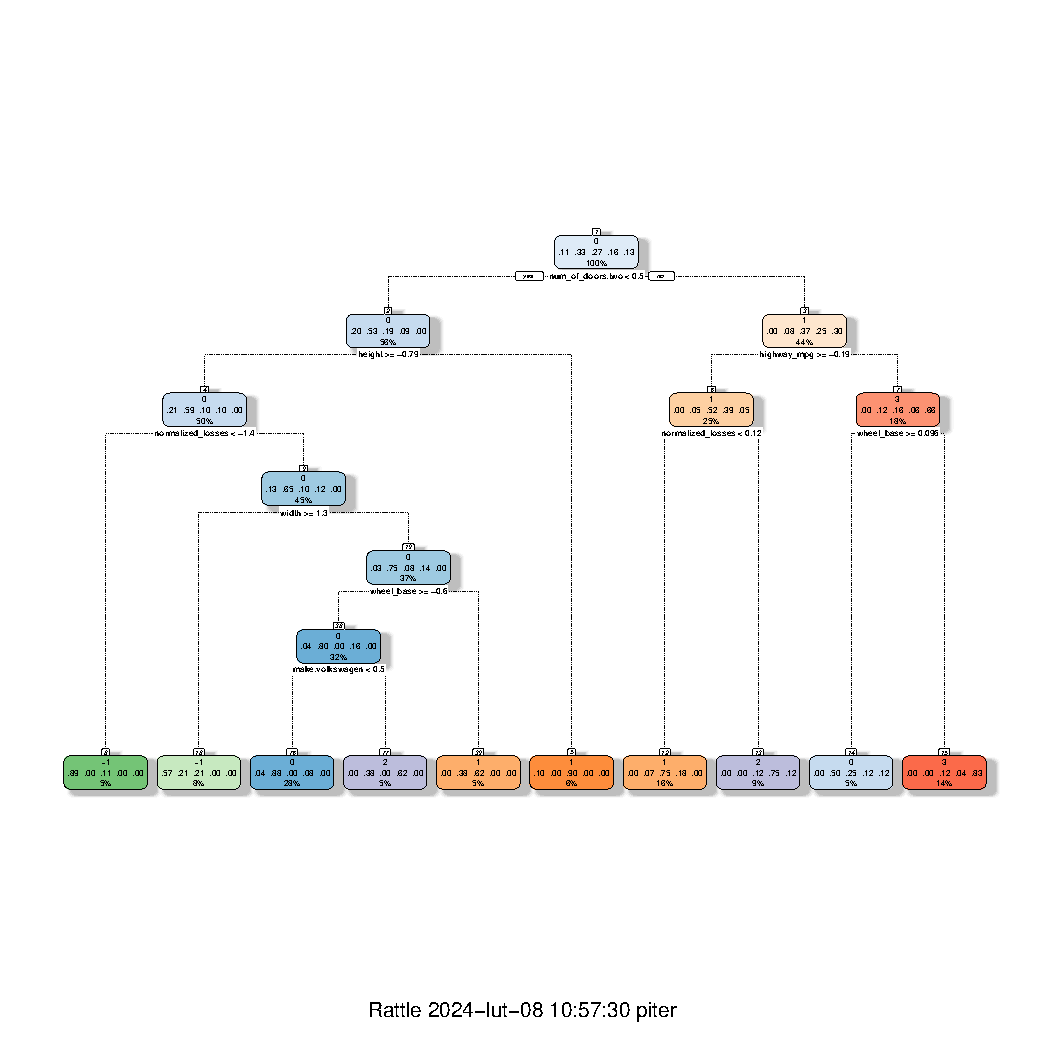
\includegraphics[width=\maxwidth]{figure/tree-1} \caption[Final tree for all features]{Final tree for all features}\label{fig:tree}
\end{figure}

\end{knitrout}

	In the figure \ref{fig:tree} we can see optimal classification tree for our classification problem. As we see, all classes are included in tree leaves. One of the big advantages of classification trees is that they are easy to interpretation for interested, for instance in our case automobile companies can easily see which parameters impact the most for certain risky ratio and what can be change to improve results.
	
Now let us see results for the most important features:
	


The best complexity parameter for our tree is equal to 0.001 and the accuracy --- 0.6884038. Below we perform a visualization of the tree:

\begin{knitrout}
\definecolor{shadecolor}{rgb}{0.969, 0.969, 0.969}\color{fgcolor}\begin{figure}
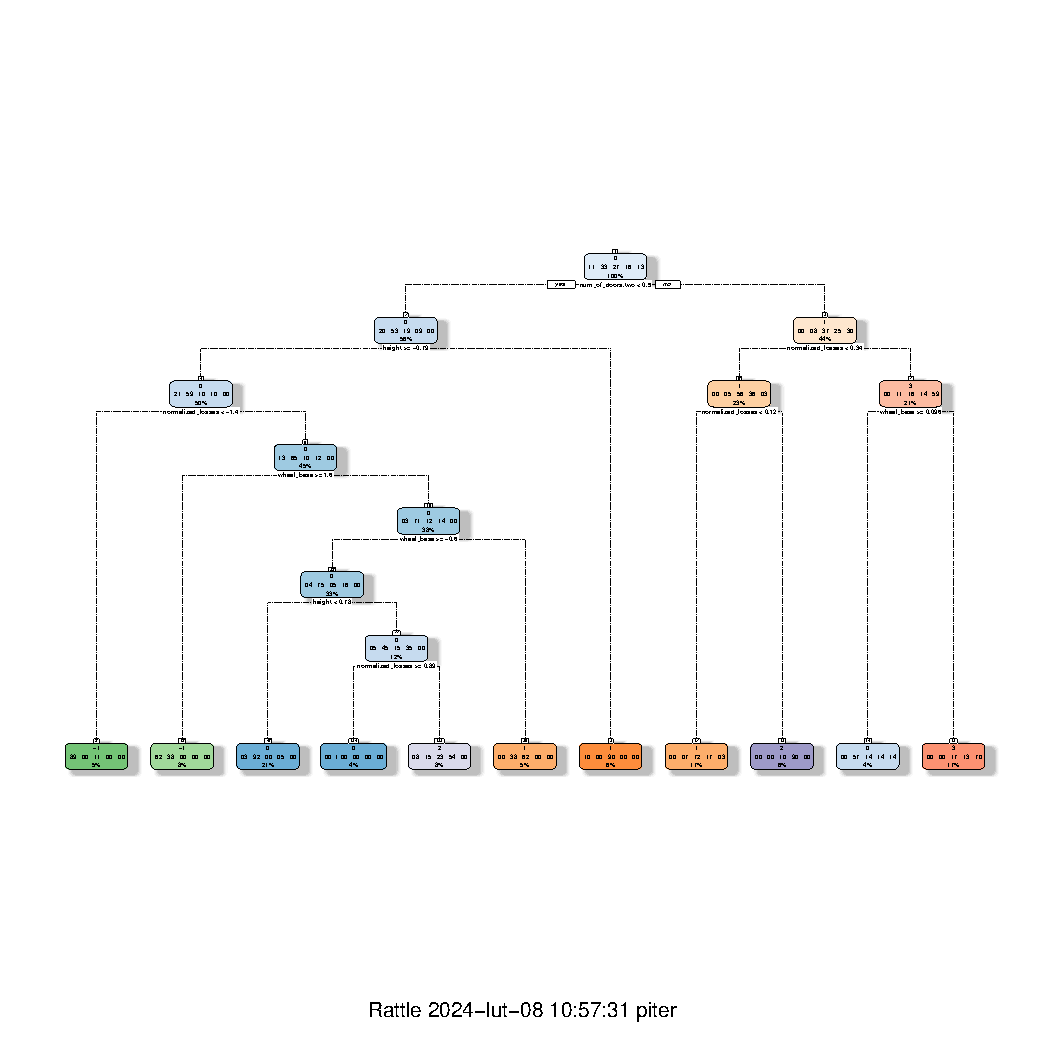
\includegraphics[width=\maxwidth]{figure/tree2-1} \caption[Final tree for most important features]{Final tree for most important features}\label{fig:tree2}
\end{figure}

\end{knitrout}
	
	\subsection{Random forest}
	Our next considered classification method is random forest. As earlier we use 5-fold Cross-Validation to assess the accuracy of classification method. We will use random forest implementation from \verb|caret| package and we will tune the number of variables randomly sampled as candidates at each split parameter. We know that there is recommended to use the number of variables randomly sampled equal to square root of number of features, so we will set the grid to this parameter in between -5 and 15 around square root of number of features in our dataset.
	

	

	
	The optimal number of variables randomly sampled as candidates at each split is equal to 18 and the accuracy for those parameter is equal to 0.7979204.
	

	
	


	In case of selected features the optimal number of variables randomly sampled as candidates at each split is equal to 2 and the accuracy for those parameter is equal to 0.8955704.
	
	\subsection{Support Vector Machine (SVM)}
	In this subsection we will apply SVM to our data. We will use implementation of SVM for \verb|caret| package, from R programming language. This package provides also automagically hyper parameter tuning for provided kernel. We will tune hyper parameters for three kernels: linear, polynomial and radial. We will use 5-fold Cross-validation to assess accuracies and we will take the kernel and correspondent hyper parameters, for which the accuracy will be the largest.
	

	
\begin{knitrout}
\definecolor{shadecolor}{rgb}{0.969, 0.969, 0.969}\color{fgcolor}\begin{kframe}
\begin{verbatim}
## # A tibble: 1 x 5
##       C Accuracy Kappa AccuracySD KappaSD
##   <dbl>    <dbl> <dbl>      <dbl>   <dbl>
## 1     1    0.748 0.669      0.102   0.134
\end{verbatim}
\end{kframe}
\end{knitrout}
	

	
\begin{knitrout}
\definecolor{shadecolor}{rgb}{0.969, 0.969, 0.969}\color{fgcolor}\begin{kframe}
\begin{verbatim}
## # A tibble: 1 x 6
##    sigma     C Accuracy Kappa AccuracySD KappaSD
##    <dbl> <dbl>    <dbl> <dbl>      <dbl>   <dbl>
## 1 0.0110    64    0.814 0.759     0.0529  0.0656
\end{verbatim}
\end{kframe}
\end{knitrout}
	

	
\begin{knitrout}
\definecolor{shadecolor}{rgb}{0.969, 0.969, 0.969}\color{fgcolor}\begin{kframe}
\begin{verbatim}
## # A tibble: 1 x 7
##   degree scale     C Accuracy Kappa AccuracySD KappaSD
##    <int> <dbl> <dbl>    <dbl> <dbl>      <dbl>   <dbl>
## 1      3   0.1     1    0.804 0.743     0.0232  0.0279
\end{verbatim}
\end{kframe}
\end{knitrout}
	
	Now let us see results for the most important features:
	
\begin{knitrout}
\definecolor{shadecolor}{rgb}{0.969, 0.969, 0.969}\color{fgcolor}\begin{kframe}
\begin{verbatim}
## # A tibble: 1 x 5
##       C Accuracy Kappa AccuracySD KappaSD
##   <dbl>    <dbl> <dbl>      <dbl>   <dbl>
## 1     1    0.660 0.544     0.0452  0.0558
\end{verbatim}
\end{kframe}
\end{knitrout}
	
\begin{knitrout}
\definecolor{shadecolor}{rgb}{0.969, 0.969, 0.969}\color{fgcolor}\begin{kframe}
\begin{verbatim}
## # A tibble: 1 x 6
##   sigma     C Accuracy Kappa AccuracySD KappaSD
##   <dbl> <dbl>    <dbl> <dbl>      <dbl>   <dbl>
## 1 0.304    32    0.833 0.781     0.0505  0.0643
\end{verbatim}
\end{kframe}
\end{knitrout}
	
\begin{knitrout}
\definecolor{shadecolor}{rgb}{0.969, 0.969, 0.969}\color{fgcolor}\begin{kframe}
\begin{verbatim}
## # A tibble: 1 x 7
##   degree scale     C Accuracy Kappa AccuracySD KappaSD
##    <int> <dbl> <dbl>    <dbl> <dbl>      <dbl>   <dbl>
## 1      3     1     4    0.793 0.729     0.0791   0.104
\end{verbatim}
\end{kframe}
\end{knitrout}
	
	As we may see in case of whole dataset we get the largest accuracy, equal to 0.8136462 for radial kernel, where sigma = 32 and C = 32 and for case of most important features we get the largest accuracy, equal to 0.832527 for radial kernel, where sigma = 32 and C = 32. We will use those hyper parameters in \ref{sec:comparison} section during results comparison.
	
	
	\section{Results comparison}\label{sec:comparison}
	In this part of project we build the model, by training whole training dataset and then we compare the results using testing dataset, which was not used during detecting the best parameters for some of the classification models. This approach allows to avoid some problems regarding correlation between fitted model and testing set.
	
	\begin{itemize}
		\item Linear regression:

		
		


The accuracy for training set is equal to 0.9248555 and for testing set --- 0.75.

For case of selected features:


		
		


The accuracy for training set is equal to 0.5202312 and for testing set --- 0.5357143.
		Feature selection has significantly less accuracy in this case.
		
		\item Logistic regression:
		

		


The accuracy for training set is equal to 0.8901734 and for testing set --- 0.7142857.

For case of selected featuers:


		


The accuracy for training set is equal to 0.5722543 and for testing set --- 0.5714286.
		Feature selection has significantly less accuracy in this case.
		\item k-Nearest Neighbors:
		


The accuracy for training set is equal to 1 and for testing set --- 0.8214286.

For case of selected features:



The accuracy for training set is equal to 1 and for testing set --- 0.7857143.
		Feature selection has a minor impact, maintaining high accuracy on both sets.
		\item Linear Discriminant Analysis:
		


The accuracy for training set is equal to 0.9537572 and for testing set --- 0.7142857.

For case of selected features:



The accuracy for training set is equal to 0.6184971 and for testing set --- 0.5714286.
	Feature selection has a notable impact, reducing accuracy on both sets.	
		
		\item Decision tree:
		




The accuracy for training set is equal to 0.7745665 and for testing set --- 0.6428571.

For case of selected features:





The accuracy for training set is equal to 0.7687861 and for testing set --- 0.4642857.
Feature selection has an impact on accuracy in case of test set, which is significantly lower, than for whole dataset, but for training sets accuracies are comparable.
		
		
		\item Random forest:
		




The accuracy for training set is equal to 1 and for testing set --- 0.8571429.

For case of selected fearures:





The accuracy for training set is equal to 1 and for testing set --- 0.7857143.
Feature selection marginally affects accuracy, maintaining strong performance.		

\item SVM:




The accuracy for training set is equal to 1 and for testing set --- 0.7857143.





The accuracy for training set is equal to 0.9942197 and for testing set --- 0.8214286.

		The SVM method demonstrated good performance on the entire dataset, achieving an accuracy of 0.7857143 using a radial kernel, sigma=1, and cost parameter C equal to 64. When considering only the most important features, the SVM method performed even better, achieving an accuracy of 0.8214286. This was achieved using a radial kernel with a sigma value of 0.304 and a cost parameter C equal to 32. The selected hyperparameters, including the kernel type, sigma, and cost parameter, significantly influenced the performance of the SVM method. The chosen parameters, such as a radial kernel with sigma=1, C=64 and a radial kernel with sigma 0.304 and C=32, proved to be effective in capturing the underlying patterns in the data.
	\end{itemize}
	
The decision to use a dedicated testing dataset not involved in the parameter tuning process is a prudent choice. This helps mitigate issues related to overfitting and provides a more accurate representation of the models' generalization capabilities.	
	The choice of classification models significantly influences their performance, with each model showcasing varying strengths and weaknesses.
Feature selection, in certain cases, impacts accuracy, highlighting the importance of considering relevant predictors.







	
	\section{Summary and further research suggestions}
	
	In this project, we conducted a comprehensive analysis of an automobile dataset using R. The key steps included exploratory data analysis (EDA), handling missing values, standardization, and employing various classification methods such as linear regression, logistic regression, decision tree, random forest, QDA, and LDA for predicting the symboling feature of automobiles. EDA revealed valuable insights into the distribution of features and potential patterns within the dataset.
Standardization of features was performed to ensure consistency and comparability across different scales, particularly benefiting models sensitive to feature scaling
Multiple classification methods were employed to predict automobile symboling, revealing varying degrees of accuracy and highlighting the importance of model selection.

We have also managed that answer all the research questions that we have stated in the introduction:

\begin{enumerate}
\item How are the numerical features correlated with each other? -- Strong positive correlations exist between city\_mpg and highway\_mpg, wheel\_base and length, engine\_size and horsepower, length and width, length and curb\_width, as well as engine\_size and curb\_width. Moderate negative correlations are observed between peak\_rpm and price, horsepower and price, compression\_ratio and highway\_mpg, length and highway\_mpg, and curb\_weight and city\_mpg. A robust positive correlation of 0.78 is noted between horsepower and engine\_size, indicating that larger engines tend to have higher horsepower. Similarly, curb\_weight and engine\_size exhibit a strong positive correlation of 0.78, suggesting that heavier vehicles tend to have larger engines. A noticeable negative correlation with highway\_mpg suggests reduced fuel efficiency as certain vehicle attributes increase.The high correlation coefficient close to 1 between city\_mpg and highway\_mpg leads to the exclusion of city\_mpg from further analysis.



\item Which features exhibit a significant number of missing values, and how should
we address them? -- "normalized\_losses", we could not remove these records due to the total number of records in the database, so we have populated them using k--NN imputation method 


\item How well do different classification methods (linear regression, logistic regression, decision tree, random forest, QDA, LDA, SVM) perform in predicting the symboling feature? -- Linear regression shows good performance but has a slightly lower accuracy on the testing set in case of whole dataset, indicating potential overfitting. Logistic regression performs well but exhibits a similar pattern of significantly lower accuracy on the testing set in case of whole dataset, suggesting some overfitting.  Method k--NN achieves perfect accuracy on the training set but shows significantly lower accuracy on the testing set, indicating potential sensitivity to overfitting. LDA demonstrates high accuracy on the training set but experiences a significant drop in accuracy on the testing set, suggesting overfitting. Decision tree performance is moderate, with a noticeable drop in accuracy on the testing set, indicating potential overfitting. Random forest achieves perfect accuracy on the training set but exhibits a slight decrease in accuracy on the testing set, suggesting some sensitivity to overfitting. For the entire dataset, the SVM model achieved perfect accuracy on the training set (100\%) and a high accuracy of 78.57\% on the testing set.
After feature selection, the SVM model continued to exhibit strong performance, with a training set accuracy of 99.42\% and a testing set accuracy of 82.14\%.
Feature selection had a marginal impact on accuracy, indicating that the SVM model maintained robust and consistent performance even when considering a subset of the most important features.


\item What are the most important features for predicting the symboling of an automobile? --  "normalized\_losses", "wheel\_base", "height", "num\_of\_doors.two"



\item Which classification algorithm yields the most accurate predictions for symboling
based on the automobile dataset? -- Random Forest demonstrates high accuracy on the training set (1), its accuracy on the testing set is also high (0.8571429). Therefore, random forest seems to be the most robust choice for predicting the "symboling" feature in this particular project.

\end{enumerate}




Further research suggestions:
\begin{itemize}
\item Investigate the use of ensemble methods such as stacking or boosting to further boost the performance of classification models.
\item Experiment with different cross--validation strategies to ensure robust model evaluation and minimize overfitting.
\item Assess the stability of feature importance across different classification models and evaluate how robust these insights are to changes in modeling techniques.
\end{itemize}






	\section*{References}
	For the project we have utilized the materials provided for the Data Mining and Machine Learning courses. 
	
\end{document}
